\chapter{Semantica della Logica Proposizionale Classica}
\section{Fondamenti della Semantica}
Per dare una definizione di semantica si utilizzano due princìpi guida: il 
\textbf{principio di bivalenza} e il \textbf{principio di verofunzionalità}. 

\begin{pri}[Bivalenza]
Un enunciato, in ogni circostanza, è o vero o falso.
\end{pri}

Il principio di bivalenza ha come conseguenza il principio del terzo escluso. 

\begin{pri}[Verofunzionalità, composizionalità o estensibilità]
Il valore di verità di un enunciato composto dipende solo dal valore di verità 
degli enunciati che lo compongono e dal significato del connettivo che li unisce. 
\end{pri}

Dato il principio di verosimiglianza, per dare la semantica ad un connettivo come $\land$ si deve dire qual è, sotto ogni circostanza, il valore di verità di $A \land B$, il quale può essere \texttt{vero} o \texttt{falso} e può dipendere solo dal valore di verità di $A$ e $B$ e dal significato fissato per $\land$. \\
\`E per questo necessario definire informalmente una \textit{circostanza} come un assegnamento che definisce lo stato vero o falso di una lettera proposizionale (o di una formula), definita come una funzione $\mathcal{v}$:
$$
\mathcal{v} : \mathscr{L} \rightarrow \{0,1\}
$$

Quindi $\mathcal{v}(A \land B) \in \{0,1\}$ e, grazie al principio di Verofunzionalità, 
dipende solo da $\mathcal{v}(A)$, 
$\mathcal{v}(B)$ e dal significato fissato per $\land$, definito come 
$$
I_{\land}: \{0,1\}^2 \rightarrow \{0,1\}
$$
E si ha, quindi
$$
\mathcal{v}(A \land B ) = I_{\land} (\mathcal{v}(A), \mathcal{v}(B))
$$
\paragraph{Importanza della Verofunzionalità}
Non è una proprietà così scontata come sembrerebbe: si supponga per un attimo che invece di Logica si stia studiando Probabilità, tentando di formalizzarla come stiamo formalizzando ora la Logica Proposizionale. \\
Si consideri una circostanza in cui due eventi hanno probabilità $p(A) = p(B) = \frac{1}{2}$. Sappiamo che la probabilità $p(A \rightarrow A) = 1$ rappresenta l'evento certo. Se valesse la proprietà verofunzionale si potrebbe dire che visto che $p(\frac{1}{2} \rightarrow \frac{1}{2}) = 1$, allora vale anche $p(A \rightarrow B) = 1$. Assurdo! \\
Per concretezza, si immagini $A = $ ``domani piove'' e $B = $ ``a Pasqua nevica''.

In conclusione, la Verofunzionalità è una caratteristica stringente della Logica Proposizionale da non dare affatto per scontata.

\subsection{Definizione di Semantica}
Siamo finalmente pronti per dare una definizione formale della 
\textbf{semantica} della Logica Proposizionale: 
\begin{defi}[Semantica della Logica Proposizionale]
Un assegnamento (o valutazione) è un'arbitraria funzione 
$$
\mathcal{v} : \mathscr{L} \rightarrow \{0,1\}
$$ 
\end{defi}
che formalizza la nozione intuitiva di circostanza (o \textit{mondo possibile}). 

\begin{defi}[Semantica dei connettivi]
        La \textbf{semantica dei connettivi} è espressa tramite delle funzioni:
$$
I_{\land} : \{0,1\}^2 \rightarrow \{0,1\}
$$
che identificano una \textit{tabella di verità}.
\end{defi}
I valori di verità dei connettivi possono anche essere espressi in forma algebrica, per esempio:
$$
\widetilde{\mathcal{v}}(A \rightarrow B) = min\{1-\widetilde{\mathcal{v}}(A), \widetilde{\mathcal{v}}(B)\}
$$

\begin{defi}[Semantica degli Enunciati]
        La \textbf{semantica degli enunciati} è l'\textbf{estensione canonica}
$$
\widetilde{\mathcal{v}}: \mathscr{F_L} \rightarrow \{0,1\}
$$
ossia l'estensione di $\mathcal{v}$ a tutte le formule, definita in questo modo: 
\begin{itemize}
  \item $\widetilde{\mathcal{v}}(p) = \mathcal{v}(p)$ se $p \in \mathscr{L}$
  \item $\widetilde{\mathcal{v}}(A \land B) = I_{\land}(\widetilde{\mathcal{v}}(A), \widetilde{\mathcal{v}}(B))$ se $p \in \mathscr{F_L}$
  \item $\widetilde{\mathcal{v}}(A \lor B) = I_{\lor}(\widetilde{\mathcal{v}}(A), \widetilde{\mathcal{v}}(B))$se $p \in \mathscr{F_L}$
  \item $\widetilde{\mathcal{v}}(A \rightarrow B) = I_{\rightarrow}(\widetilde{\mathcal{v}}(A), \widetilde{\mathcal{v}}(B))$ se $p \in \mathscr{F_L}$
  \item $\widetilde{\mathcal{v}}(\neg A) = I_{\neg}(\widetilde{\mathcal{v}}(A))$ se $p \in \mathscr{F_L}$
\end{itemize}
\end{defi}

Con un poco importante abuso notazionale, si tenderà ad evitare di esplicitare 
$\widetilde{\mathcal{v}}$ in favore della notazione $\mathcal{v}$.
\section{Nozioni Semantiche Fondamentali}

\begin{defi}[Tautologia]
Una formula $F \in \mathscr{F_L}$ è una \textit{tautologia} se e solo se 
$$
\forall \widetilde{\mathcal{v}} : \mathscr{F_L} \rightarrow \{0,1\} ~~~ \widetilde{\mathcal{v}}(F) = 1
$$
\end{defi}
\begin{defi}[Formula Soddisfacibile]
Una formula $F \in \mathscr{F_L}$ è \textit{soddisfacibile} se e solo se 
$$
\exists \widetilde{\mathcal{v}} : \mathscr{F_L} \rightarrow \{0,1\} : \widetilde{\mathcal{v}}(F) = 1
$$
\end{defi}
\begin{defi}[Contraddizione]
Una formula $F \in \mathscr{F_L}$ è una \textit{contraddizione} (o insoddisfacibile, refutabile) se e solo 
se 
$$
\forall \widetilde{\mathcal{v}} : \mathscr{F_L} \rightarrow \{0,1\} ~~~ \widetilde{\mathcal{v}}(F) = 0
$$
\end{defi}
C'è un fatto molto semplice che lega tra di loro questi concetti: 
\begin{teo}
$F \in \mathscr{F_L}$ è una tautologia se e solo se $\neg F$ è insoddisfacibile. 
\end{teo}
\begin{proof}
  \begin{align*}
         & F \text{ tauto} \\
    \iff & \widetilde{\mathcal{v}}(F) = 1 ~~~ \forall \widetilde{\mathcal{v}} : \mathscr{F_L} \rightarrow \{0,1\} & \text{per def. di tauto}\\
    \iff & \widetilde{\mathcal{v}}(\neg F) = 0 ~~~ \forall \widetilde{\mathcal{v}} : \mathscr{F_L} \rightarrow \{0,1\} & \text{per def. } I_{\neg} \\
    \iff & \neg F \text{ insodd.} & \text{per def. di contraddizione}
  \end{align*}
\end{proof}

\subsection{Principio d'Induzione su $\mathscr{F_L}$}
Benché non sia una sfaccettatura prettamente semantica, in quanto verrà (anzi, è già stato) utilizzato abbondantemente, è importante formalizzare il  \textbf{principio d'induzione}. Sia $P$ una proprietà delle formule; si ha che $P$ vale per ogni formula $F \in \mathscr{F_L}$ se e solo se:
\begin{itemize}
  \item \textbf{base} ($F = p$): $P$ vale per ogni $p \in \mathscr{L}$
  \item \textbf{passo}: se $P$ vale per $A,B  \in \mathscr{F_L}$, allora 
    vale anche per $\neg A$, $A \rightarrow B$, $A \lor B$ e $A \land B$. 
\end{itemize}

Una proprietà si può dimostrare induttivamente anche grazie alla definizione  induttiva di $\mathscr{F_L}$. Sia:
$$
I = \{ F \in \mathscr{F_L} : \text{ la proprietà } P \text{ vale per } F\}
$$
Si vuole mostrare $I = \mathscr{F_L}$, ossia che $I$ è esattamente l'insieme di tutte le formule. Questo si fa mostrando che $I \subseteq \mathscr{F_L}$ (ovvio per def. di $I$) e che $\mathscr{F_L} \subseteq I$, come segue.
\begin{proof}
$I$ soddisfa il primo e il secondo punto della definizione induttiva di $\mathscr{F_L}$ perché contiene tutte le lettere proposizionali (base) e, induttivamente le formule composte da sottoformule $A,B \in I$. Allora $I$ conterrà anche $(\neg A)$, $(A \rightarrow B)$, $(A \land B)$ e $(A \lor B)$. \\
Grazie al terzo punto della definizione, invece, si può affermare che $I = \mathscr{F_L}$ in quanto non sono contenute altre formule in $I$ (per definizione).
\end{proof}

Come esempio, si dimostra induttivamente il seguente lemma: 
\begin{lem}[Verità di una Formula]
Sia $F \in \mathscr{F_L}$ e siano $\mathcal{v}, \mathcal{v}' : \mathscr{L} \rightarrow \{0,1\}$. 

Se $\mathcal{v}(p) = \mathcal{v}'(p) \forall p \in \mathscr{L} \in F$\footnote{Per ogni letterale nell'insieme dei letterali nella formula.}, 
allora $\widetilde{\mathcal{v}}(F) = \widetilde{\mathcal{v}}'(F)$.
\end{lem}
\begin{proof}
  \textit{Per induzione su } $\mathscr{F_L}$.
  \begin{itemize}
    \item \textbf{base} ($F = p \in \mathscr{L}$): 
      \begin{align*}
        & \mathcal{v}(p) = \mathcal{v}'(p) \\
        \iff & \widetilde{\mathcal{v}}(p) = \widetilde{\mathcal{v}}'(p) & \text{per def. }\widetilde{\mathcal{v}}
      \end{align*}
    \item \textbf{passo}:
    \begin{itemize}
      \item $F = \neg A$:
        \begin{align*}
          \widetilde{\mathcal{v}}(F) &= 1 - \widetilde{\mathcal{v}}(A) & \text{per def. } \widetilde{\mathcal{v}} \text{ e } I_\neg \\
          &= 1 - \widetilde{\mathcal{v}}'(A) & \text{per I.H.} \\
          &= \widetilde{\mathcal{v}}'(F) & \text{per def. } \widetilde{\mathcal{v}} \text{ e } I_\neg
        \end{align*}
      \item Se $F = (A \land B)$:
        \begin{align*}
          \widetilde{\mathcal{v}}(F) &= \min\{\widetilde{\mathcal{v}}(A), \widetilde{\mathcal{v}}(B)\} & \text{per def. } \widetilde{\mathcal{v}} \text{ e } I_\land \\
          &= \min\{\widetilde{\mathcal{v}}'(A), \widetilde{\mathcal{v}}'(B)\} & \text{per I.H.} \\
          &= \widetilde{\mathcal{v}}'(F) & \text{per def. } \widetilde{\mathcal{v}} \text{ e } I_\land        
        \end{align*}
      \item uguale per gli altri connettivi.
    \end{itemize}
  \end{itemize}
\end{proof}
Il lemma appena provato ci garantisce che se vogliamo calcolare $\widetilde{\mathcal{v}}(F)$ 
ci basta calcolare la tabella di verità di $F$. A questo punto si può calcolare, 
per ogni assegnamento, se una formula è vera, soddisfacibile, tautologica o 
insoddisfacibile.

\paragraph{Esercizio}
Date $A, B \in \mathscr{F_L}$ si esaminino le seguenti formule. 
La formula $A \land \neg A$ è insoddisfacibile, come si può osservare dalla 
sua tabella di verità nella Tabella \ref{table:insodd}.
\begin{table}[!h]
  \centering
  \begin{tabular}{|c|c|}
  \hline
  $A$ & $A \land \neg A$ \\
   0  &   0        \\ 
   1  &  0         \\
   \hline
 \end{tabular}
 \caption{}
 \label{table:insodd}
\end{table}

La formula $A \rightarrow \neg A$ è soddisfacibile ma non tautologica, 
come si può osservare dalla sua tabella di verità nella Tabella \ref{table:sodd}.
\begin{table}[h]
  \centering
  \begin{tabular}{|c|c|}
    \hline 
    $A$ & $A \rightarrow \neg A$\\
     0 &   1 \\
     1 &  0 \\
     \hline
  \end{tabular}
  \caption{}
  \label{table:sodd}
\end{table}

Si noti come è stato detto che $A,B$ siano state definite come appartenenti 
all'insieme delle formule e non alle lettere ($L$), ``imbrogliando'', un poco, 
rispetto al lemma precedente. Tuttavia, $A$ e $B$ possono essere considerate 
come \textit{metavariabili} a prescindere dalla loro complessità. Non è invece 
possibile fare il contrario, ossia considerare lettere come delle formule: 
per esempio, non è possibile dire che una lettera sia una tautologia. 

\paragraph{Esercizio}
Verificare che le seguenti siano Tautologie per ogni $A,B \in \mathscr{F_L}$:
\begin{enumerate}
  \item $A \rightarrow (B \rightarrow A)$ (Weakening, Prefixing)
  \item $(\neg A \rightarrow A) \rightarrow A$ (Consequentia Mirabilis)
  \item $(A \rightarrow B) \lor (B \rightarrow A)$ 
  \item $(A \rightarrow B) \rightarrow (\neg B \rightarrow \neg A)$ (Contronominale)
  \item $(A \land B) \rightarrow A$
  \item $A \lor \neg A$  (Tertium non datur)
  \item $\bot \rightarrow A$ (Ex Falsum Quodlibet Sequitur)
\end{enumerate}

\begin{defi}[Tautologia]
Se la formula $F$ è una tautologia, si indicherà 
$$
\models F
$$
\end{defi}


\section{Semantica degli Insiemi di Formule}
\begin{defi}[Teoria]
Sia $\Gamma \subseteq \mathscr{F_L}$ un insieme di formule. $\Gamma$ è detto 
\textbf{teoria} ed è un modello per un mondo in cui tutte le formule che 
gli appartengono sono vere.
\end{defi}
Si dice che $\Gamma$ è soddisfacibile ($\mathcal{v} \models \Gamma$) se e solo se  
$$
\exists \mathcal{v}: \mathscr{L} \rightarrow \{0,1\} ~~~ \forall \gamma \in \Gamma:\mathcal{v}(\gamma) = 1
$$
o, in notazione alternativa, $\mathcal{v} \models \gamma$. \\
Al contrario, la teoria $\Gamma$ è insoddisfacibile ($\mathcal{v} \nvDash \Gamma$) se e solo se 
$$
\forall \mathcal{v}: \mathscr{L} \rightarrow \{0,1\} ~~ \exists \gamma \in \Gamma : \mathcal{v} \nvDash \gamma
$$

\begin{defi}[Conseguenza Logica]
Sia $\Gamma \subseteq \mathscr{F_L}$ e $A \in \mathscr{F_L}$. La formula $A$ è una 
\textbf{conseguenza logica} di $\Gamma$ se e solo se 
$$
\forall \mathcal{v} : \mathcal{v} \models\Gamma,\ \mathcal{v} \models A
$$ 
Si denoterà questo fatto con la notazione $\Gamma \models A$.
\end{defi}

\paragraph{Esercizio} 
Esprimere il concetto di formula tautologica o tautologia ($\models A$)
attraverso il concetto di conseguenza logica. \\
Quando si ammette una teoria, si restringe il campo dei possibili assegnamenti. 
Una formula è tautologica quanto è vera in ogni circostanza ed è verificata 
da ogni assegnamento. Sia $\Gamma$ definito in questo modo. $\Gamma \subseteq \mathscr{F_L}$ 
un insieme composto solo da tautologie. Allora 
$\Gamma \models A$. Dato che è sempre meglio avere come teoria la più semplice 
possibile, si può definire $\Gamma = \emptyset$, concludendo $\emptyset \models A$. 

\noindent
Ogni tanto si può utilizzare la notazione $\Gamma \cup \{A\} \models B$, che 
a volte viene semplificato in $\Gamma,A \models B$. 

\subsection{Proprietà semantiche fondamentali delle Teorie}

\begin{lemn}[Conseguenza Logica di una Formula da una Teoria insoddisfacibile]
\label{lem:conseguenza-teoria-insodd-formula}
Sia $\Gamma \subseteq \mathscr{F_L}$ una teoria e $A \in \mathscr{F_L}$. Si 
ha che $\Gamma \models A$ se e solo se $\Gamma \cup \{\neg A \}$ è insoddisfacibile. 
\end{lemn}

\begin{proof}
\begin{align*}
  & \Gamma \models A \\
  \iff & \forall \mathcal{v} ~~~ (\forall \gamma \in \Gamma,\ \mathcal{v} \models \gamma) \text{ implica } \mathcal{v} \models A & \text{per def. } \models \\
  \iff & \forall \mathcal{v} ~~~ \neg (\forall \gamma \in \Gamma,\ \mathcal{v} \models \gamma) \lor \mathcal{v}\models A & \text{implicazione materiale} \\
  \iff & \forall \mathcal{v} ~~~ \neg (\forall \gamma \in \Gamma,\ \mathcal{v}(\gamma) = 1) \lor \mathcal{v}(A) = 1\\
  \iff & \forall \mathcal{v} ~~~ (\exists \gamma \in \Gamma : \mathcal{v}(\gamma) = 0) \lor \mathcal{v}(\neg A) = 0 \\
  \iff & \forall \mathcal{v} ~~~ \exists B \in \Gamma \cup \{\neg A\} \text{ t.c. } \mathcal{v}(B) = 0  \\
  \iff & \Gamma \cup \{\neg A\} \text{ è insodd.} & \text{per def. insodd.}
\end{align*}
\end{proof}

\begin{lemn}[Lemma semantico o di deduzione]
\label{lem:deduzione}
Siano $P$, $Q$ due formule. Allora si dice che $P \models Q$ se e solo se $\models P \rightarrow Q$. 
\end{lemn}
\begin{proof}
Assumiamo che $P \models Q$.\\
Per definizione, 
$\forall \mathcal{v}: \mathscr{L} \rightarrow \{0,1\}:\mathcal{v}(P) = 1$ implica $\mathcal{v}(Q) = 1$. 
È quindi chiaro che ogni volta che $\mathcal{v}(P) = 1$, si ha $\mathcal{v}(Q) = 1$; è perciò impossibile avere $P$ vero e $Q$ falso. Ne segue che $\models P\rightarrow Q$ è una tautologia, per definizione di $I_\rightarrow$.
\end{proof}

Il teorema generalizza il lemma alla seguente situazione. 
\begin{teo}[Thm. semantico o di deduzione]
\label{thm:deduzione}
Sia $\Gamma$ una teoria 
e $P$, $Q$ formule. Allora $\Gamma,P \models Q$ se e solo se
$\Gamma \models P \rightarrow Q$. 
\end{teo}
\begin{proof}
\begin{align*}
  &\Gamma, P \models Q \\
  \iff & \forall \mathcal{v} ~~~ ((\forall \gamma \in \Gamma, \mathcal{v}(\gamma) = 1) \land \mathcal{v}(P) = 1) \rightarrow \mathcal{v}(Q) = 1 & \text{per def. } \models \\
  \iff & \forall \mathcal{v} ~~~ (\forall \gamma \in \Gamma, \mathcal{v}(\gamma) = 1) \rightarrow \mathcal{v}(P \rightarrow Q) = 1 & A \land B \rightarrow C \equiv A \rightarrow (B \rightarrow C) \\
  \iff & \Gamma \models P \rightarrow Q & \text{per def. di } \models
\end{align*}
\end{proof}

\subsection{Teorema di Compattezza}
Il teorema di compattezza è un teorema fondamentale della logica e varrà 
anche per la logica del primo ordine. Lo proviamo ora per la logica proposizionale. 
\`E in qualche modo, in forma astratta, un teorema di completezza. 

Prima di mostrare l'enunciato, si introduce il concetto. \`E stata data la 
nozione di teoria, $\Gamma \subseteq \mathscr{F_L}$: ci si chiede se serve, nella logica 
proposizionale, considerare teorie infinite (composte da un numero 
infinito di formule). A priori, sembrerebbe proprio di sì - d'altronde $\mathscr{F_L}$ è di 
cardinalità numerabile - e si vedrà affrontando
la Logica dei Predicati che una singola formula al primo ordine contiene informazioni 
di un numero infinito di formule proposizionali; questo basta per giustificare il caso 
in cui $\Gamma$ sia una teoria infinita. Il punto è che non sembra possibile 
gestire la teoria infinita: qui torna utile il teorema di compattezza. 
 

Il teorema di compattezza permette di ridurre l'analisi della soddisfacibilità di 
una teoria eventualmente infinita all'esame della soddisfacibilità dei suoi 
sottoinsiemi finiti. Tuttavia, è ovvio che il numero di sottoinsiemi finiti 
sia infinito. 
\noindent

\begin{defi}
        $\Gamma$ \textit{è finitamente soddisfacibile} (fin. sodd.) 
        se $\forall \Gamma' \subseteq_{\omega} \Gamma$ (leggasi ``$\Gamma '$ sottoinsieme finito di $\Gamma$'')
        si ha che $\Gamma'$ è soddisfacibile.
\end{defi}

\begin{teon}[di Compattezza]
\label{thm:compattezza-prop}
$\Gamma \subseteq \mathscr{F_L}$ è soddisfacibile $\iff \Gamma'$ è soddisfacibile $\forall \Gamma' \subseteq_{\omega} \Gamma$.
\end{teon}
$\Gamma$ è soddisfacibile $\implies \Gamma'$ è soddisfacibile $\forall \Gamma' \subseteq \Gamma$ è ovvio per definizione di soddisfacibilità di una teoria.

\subsubsection{Dimostrazione ($\Longleftarrow$)}
Il succo della dimostrazione sarà la relazione tra finitamente soddisfacibile e soddisfacibile: vogliamo provare $\Gamma$ fin. sodd. $\implies \Gamma$ soddisfacibile. 

Fissato una successione senza ripetizioni di tutte le formule in $F_i \in \mathscr{F_L}$:
$$
F_1, F_2, \cdots, F_k, \cdots
$$ 
si costruisce una successione infinita di insiemi di formule:
$$
D_0, D_1, \cdots, D_k, \cdots
$$ 
definita induttivamente sull'indice $i$ di $D_i$:
\begin{itemize}
  \item \textbf{base}: $D_0 = \Gamma$
  \item \textbf{passo}: $D_{n+1} = 
        \begin{cases} 
          D_n \cup \{F_{n+1}\} & \text{se } D_n \cup \{F_{n+1}\} \text{ è finitamente soddisfacibile} \\
          D_n \cup \{\neg F_{n+1}\} & \text{altrimenti}
        \end{cases}$
\end{itemize}


Bisogna sottolineare che la definizione di $D_n$ non garantisce, a priori, 
che ogni $D_n$ sia finitamente soddisfacibile, anche se si dimostrerà che è 
in effetti così. In altre parole, definire $D_n = D_{n-1} \cup \{\neg F_{n+1}\}$ 
se l'alternativa non è finitamente soddisfacibile, non ci assicura a priori che 
$D_n$ sia fin. sodd.; per arrivare a tale conclusione è necessaria una 
dimostrazione.
Si definisce infine
$$
D = \bigcup_{i \in \mathbb{N}} D_i
$$
Prima di passare alle effettive dimostrazioni, si noti come per dimostrare 
una proprietà di $\Gamma$ stiamo cercando di dimostrare qualcosa di relativo a 
un insieme infinitamente più grande, $D$; benché questa possa sembrare un'idea 
balzana, il Teorema di Compattezza ci dimostrerà che questo è il procedimento 
giusto per ottime ragioni. 

\paragraph{Fatto 1:}
\textit{$D_n$ è finitamente soddisfacibile $\forall n$.}

\begin{proof}
Per induzione su $n$:
\begin{itemize}
  \item \textbf{base}: $D_0 = \Gamma$ è finitamente soddisfacibile per ipotesi.
  \item \textbf{passo} $D_{n+1}$: per assurdo, assumiamo $D_{n+1}$ non finitamente soddisfacibile.
  \begin{align*}
    \iff & \exists D' \subseteq_{\omega} D_{n}\cup \{F_{n+1}\} \text{ tale che } D' \text{ è insoddisfacibile} & (1)\\
    \text{e}\ & \exists D''\subseteq_{\omega} D_{n} \cup \{\neg F_{n+1}\} \text{ tale che } D''   \text{ è insoddisfacibile} & (2)
  \end{align*}
  Senza perdita di generalità, si può assumere che:
  \begin{align*}
    & F_{n+1} \in D' \text{ e } \neg F_{n+1} \in D'' & \text{perchè }D_n \text{ è sodd. per ipotesi induttiva}\\
    \iff & D' = E' \cup \{F_{n+1}\} \text{ e } D'' = E'' \cup \{\neg F_{n+1}\}
    & \text{ con } E', E'' \subseteq_\omega D_{n} : F_{n+1} \notin E', \neg F_{n+1} \notin E''\\
    \iff & D' \subseteq E' \cup E'' \cup \{F_{n+1}\} \text{ e } & \text{insod. per }(1)\\
    & D'' \subseteq E' \cup E'' \cup \{\neg F_{n+1}\} & \text{insod. per }(2)
  \end{align*}
  Ma $E' \cup E'' \subseteq_{\omega} D_{n}$ e per ipotesi induttiva $D_n$ è finitamente soddisfacibile, ed è quindi $E' \cup E''$ soddisfacibile ed esiste un assegnamento tale che $\mathcal{v} \models E' \cup E''$. Sappiamo che $\mathcal{v}(F_{n+1})$ è uguale a $0$ o a $1$ e pertanto non è possibile che entrambi $\{F_{n+1}\}$ e $\{\neg F_{n+1}\}$ siano falsi. Abbiamo raggiunto la contraddizione che conclude la prova per assurdo mostrando $D_{n+1}$ finitamente soddisfacibile. Questo chiude a sua volta la prova per induzione, mostrando che ogni $D_n$ per $n \in N$ è finitamente soddisfacibile. 
  \end{itemize}
\end{proof}
 
\paragraph{Fatto 2:}
\textit{$D = \bigcup\limits_{i \in \omega} D_i$ è a sua volta finitamente 
soddisfacibile.}

Questo non è necessariamente ovvio a partire dal fatto 
che $D = \bigcup\limits_{i \in \omega} D_i$ con $D_i$ fin. sodd.\\
\begin{proof}
Siano:
\begin{itemize}
  \item $D' \subseteq_{\omega} D$, un sottoinsieme finito qualunque, con $D' = \{F_{i_1}, F_{i_2},\cdots,F_{i_u}\}$
  \item $k = \max\limits_{j=1,...,u} i_j$, l'indice massimo
\end{itemize}
Allora:
\begin{align*}
  & D' \subseteq_{\omega} D_k\\
  \implies & D' \text{ è finitamente soddisfacibile} & \text{per Fatto 1} \\
  \implies & D \text{ è finitamente soddisfacibile} & \text{quando } D' = D
\end{align*}
\end{proof}

\paragraph{Fatto 3:}
\textit{Per ogni formula o enunciato $F_t$ esattamente \textbf{una} tra $F_t$ e $\neg F_t$ appartiene a $D$.}

Anche questo non è necessariemente garantito, in quanto $F_t$ e $\neg F_t$ non hanno lo stesso indice, ossia $\neg F_t$ non ha indice $t$.\\
\begin{proof}
Per costruzione della sequenza di $D_i$:
\begin{align*}
  & F_t \in D_t \vee \neg F_t \in D_t\\
  \implies & F_t \in D \vee \neg F_t \in D & \text{dato che ogni } D_t \subseteq D
\end{align*}
Si può escludere che ci siano entrambe: $\{F_t, \neg F_t\} \nsubseteq D$. Infatti, per assurdo:
\begin{align*}
  & \{F_t, \neg F_t\} \subseteq D\\
  \implies & D \text{ è fin. sodd.} & \text{per Fatto 2}\\
  \implies & \{F_t, \neg F_t\} \text{ è sodd.} & \text{per def. fin. sodd.} \\
  \implies & \bot & \text{per la semantica della negazione } I_\neg
\end{align*}
\end{proof}

\paragraph{Fatto 4:}
\textit{Sia $\mathcal{v}_D : \mathscr{L} \rightarrow \{0,1\}$ t.c. $\forall p \in \mathscr{L},\ \mathcal{v}_D(p) = 1 \iff p \in D$. Allora:}
$$
  \mathcal{v}_D \models D
$$
\textit{Ovvero} $\forall F \in D,\ \widetilde{\mathcal{v}}_D(F) = 1$

Si noti che $\mathcal{v}_D$ è \textit{ben definito} in quanto necessariamente $p \in D$ o $p \notin D$.

\begin{proof}
Per induzione strutturale proviamo la coimplicazione:
$$
  \forall F \in \mathscr{F_L},\ \widetilde{\mathcal{v}}_D(F) = 1 \iff F \in D
$$
Questo non è uguale alla definizione precedente, in quanto 
in principio è stato definito per le lettere proposizionali e non per la 
funzione estesa ($\widetilde{\mathcal{v}}_D$). Ci basterebbe provare che $F \in D$ 
implica $\mathcal{v}_D(F) = 1$ ma per convenienza proviamo anche che 
$\mathcal{v}_D(F) = 1$ implica $F \in D$. 
\begin{itemize}
  \item \textbf{base}: $F = p$, con $p \in \mathscr{L}$
  \begin{align*}
    \mathcal v_D(F) = 1 \iff \mathcal v_D(p) \iff p \in D \iff F \in D \text{ per definizione di }\mathcal{v}_D
  \end{align*}
  \item \textbf{passo}:
    \begin{itemize}
      \item se $F = \neg G: $
        \begin{align*}
          & \mathcal{v}_D(F) = 1 \\
          \iff & \mathcal v_D(\neg G) = 1 \\
          \iff & \mathcal{v}_D(G) = 0 & \text{per def. di }I_\neg\\
          \iff & G \notin D & \text{per ipotesi induttiva}\\
          \iff & \neg G \in D & \text{per Fatto 3} \\
          \iff & F \in D
        \end{align*}
      \item se $F = (G \land H):$
        \begin{align*}
          & \mathcal{v}_D(F) = 1 \\
          \iff & \mathcal{v}_D(G \land H) = 1 \\
          \iff & \mathcal{v}_D(G) = 1 \land \mathcal{v}_D(H) = 1 & \text{per def. di }I_\land \\
          \iff & G \in D \land H \in D & \text{per ipotesi induttiva} \\
          \iff & (G \land H) \in D
        \end{align*}
        L'ultima implicazione è dimostrabile per assurdo:
        \begin{align*}
          & (G \land H) \notin D & \text{deduzione assurda (} \Rightarrow \text ) \\
          \implies & \neg(G \land H) \in D & \text{per Fatto 3} \\
          \implies & \{G, H, \neg (G \land H)\} \subseteq_{\omega} D \text{ fin. sodd.} & \text{per Fatto 2, ma } \bot \text{ per } I_\neg, I_\land \\[5pt]
          & G \notin D \lor  H \notin D & \text{deduzione assurda (} \Leftarrow \text ) \\
          \implies & \text{se } G \notin D:\ \neg G \in D & \text{per Fatto 3} \\
          & \{G \land H, \neg G\} \subseteq_{\omega} D \text{ fin. sodd.} & \text{ per Fatto 2, ma } \bot \text{ per } I_\neg, I_\land \\
          & \text{se } H \notin D:\ \neg H \in D & \text{per Fatto 3} \\
          & \{G \land H, \neg H\} \subseteq_{\omega} D \text{ fin. sodd.} & \text{ per Fatto 2, ma } \bot \text{ per } I_\neg, I_\land
        \end{align*}
      \item se $F = (G \lor H):$
          \begin{align*}
            & \mathcal{v}_D(F) = 1 \\
            \iff & \mathcal{v}_D(G \lor H) = 1 \\
            \iff & \mathcal{v}_D(G) = 1 \lor \mathcal{v}_D(H) = 1 & \text{per def. di }I_\lor \\
            \iff & G \in D \lor H \in D & \text{per ipotesi induttiva} \\
            \iff & (G \lor H) \in D
          \end{align*}
          L'ultima implicazione è dimostrabile per assurdo:
          \begin{align*}
              &(G \lor H) \notin D & \text{deduzione assurda(} \Rightarrow \text ) \\
            \implies & \neg (G \lor H) \in D & \text{per Fatto 3} \\
            \implies & \text{se } G \in D:\ \{G, \neg (G \lor H)\} \subseteq_{\omega} D \text{ fin. sodd.} & \text{per Fatto 2, ma }\bot \\
            & \text{se } H \in D:\  \{H, \neg (G \lor H)\} \subseteq_{\omega} D \text{ fin. sodd.} & \text{per Fatto 2, ma } \bot \\[5pt]
            & \neg(G \in D \lor H \in D) & \text{deduzione assurda (} \Leftarrow \text )\\
            \implies & G \notin D \land H \notin D & \text{per De Morgan}\\
            \implies & \neg G \in D \land \neg H \in D & \text{per Fatto 3}\\
            \implies & \{\neg G, \neg H, \{G \lor H \}\} \subseteq_{\omega} D \text{ fin. sodd. }& \text{per Fatto 2, ma } \bot
          \end{align*}
       \item se $F = (G \rightarrow H): $ \textit{uguale, usa il fatto che è vero se G è falso o H è vero }
    \end{itemize}
\end{itemize}
\end{proof}

Ora che abbiamo dimostrato che, se $\Gamma$ è fin. sodd., esiste un assegnamento $\mathcal v_D : \mathcal v_D \models D$, abbiamo dimostrato anche che $\mathcal v_D \models \Gamma$ (dato che $\Gamma \subseteq D$).\\
$\Gamma$ è dunque soddisfacibile.

\subsubsection{Contronominale}
Noi useremo per lo più la versione \textit{contronominale} del Teorema di Compattezza:\\
$\Gamma$ insoddisfacibile $\implies \exists \Gamma' \subseteq_{\omega} \Gamma : \Gamma'$ insoddisfacibile. 

\subsection{Osservazioni sul Teorema di Completezza}
La dimostrazione del Teorema di Compattezza lavora ampliando al massimo la teoria $\Gamma$ che si vuole analizzare:
$$
\Gamma = D_0 \subseteq D_1 \subseteq D_2 \cdots \subseteq D_k \cdots \subseteq D
$$

\begin{defi}[Insieme massimamente soddisfacibile]
  Un sottoinsieme di formule $E \subseteq \mathscr{F_L}$ è \textbf{massimamente soddisfacibile} sse 
$E$ è sodd. e $\forall F \in \mathscr{F_L} : F\notin E$ si ha che $E \cup \{F\}$ è insodd. 
\end{defi}

\begin{ossn}
$D$ è un \textbf{ampliamento massimale} di $\Gamma$, in quanto se $\overline{D} = D \cup \{F\}$ con $F \notin D$ allora $\overline D$ è insoddisfacibile per Fatto 3 ($\neg F \in D$).
\end{ossn}
$D$ è solo \textit{uno} degli ampliamenti massimali possibili, ed è quello che è stato 
costruito a partire da $\Gamma$ e da una regola di costruzione di $D_{n+1}$ non univoca che dipende dall'elenco delle formule (i.e., può succedere che, dato un letterale $p$, sia $D_n \cup \{p\}$ sia $D_n \cup \{\neg p\}$ siano sodd.).

\begin{ossn}
A livello delle informazioni contenute, un insieme massimale soddisfacibile $D$ si comporta come un assegnamento (e viceversa).
\end{ossn}
Per ogni assegnamento $\mathcal{v} : \mathscr{L} \rightarrow \{0,1\}$ si può creare $D_\mathcal{v} = \{ F \in \mathscr{F_L} : \mathcal{v}(F) = 1\}$ massimamente soddisfacibile.

\paragraph{Utilizzo}
Il Teorema di Compattezza verrà usato per decidere quando $\Gamma \stackrel{?}{\models} A$ ($A$ è conseguenza logica di $\Gamma$), problema fondamentale della logica proposizionale e del primo ordine.\\
Si usa nella sua forma contronominale assieme al Lemma~\ref{lem:conseguenza-teoria-insodd-formula}:
$$
\Gamma \models A \iff \Gamma \cup \{\neg A \} \text{ insodd.} \iff \exists \Gamma' \subseteq_{\omega} \Gamma : \Gamma' \text{ insoddisfacibile}
$$
La deduzione automatica sono infatti quei metodi refutazionali che mirano a dimostrare l'isoddisfacibilità di una teoria o di una singola formula.

Si supponga che $\Gamma$ sia una teoria finita ($\Gamma = \{B_1, \cdots, B_n\}$) e che si voglia sapere se $\Gamma \stackrel{?}{\models} A$.
\begin{align*}
  & \Gamma \models A \\
  \iff & B_1, \cdots, B_n \models A \\
  \iff & \{B_1, \cdots,B_n,\neg A\} \text{ insodd.} & \text{(come teoria)}\\
  \iff & B_1 \land \cdots B_n \land \neg A \text{ insodd.} & \text{ (come formula)}
\end{align*}
Decidere se la formula finale è sodd. o insodd. è NP-completo e si può parzialmente risolvere con i SAT-solver.

Se, invece, $\Gamma$ è infinito non si può più risolvere la soddisfacibilità come formula. È qua che si utilizza il Teorema di Compattezza: partendo da un $\Gamma_0 = \emptyset$ si cerca il $\Gamma_i \subseteq_{\omega} \Gamma : \Gamma_i$ è insodd. Se si trova allora anche $\Gamma$ è insodd.\\
Tuttavia non c'è un criterio \textit{generale} per sapere se $\Gamma$ è sodd. in tempo finito.

\section{Equivalenza Semantica}
I seguenti enunciati:
\begin{align*}
  A \lor B & & B \lor A
\end{align*}
sono due formule \textit{sintatticamente} differenti perché sono stringhe di simboli scritte diversamente.\\
Il loro \textbf{significato}, tuttavia, è uguale e, pertanto, per ogni $\mathcal{v} : \mathscr{L} \rightarrow \{0,1\}$ si ha che:
$$
\mathcal{v}(A \lor B) \equiv \mathcal{v}(B \lor A)
$$
Quella appena definita è una \textbf{relazione}. 

\begin{defi}[Relazione $n$-aria]
$R \subseteq S^{n}$ è una relazione $n$-aria su un insieme $S$.
\end{defi}
È un sottoinsieme dell'insieme di tutte le $n$-ple di elementi di $S$, in altre parole $R \subseteq S^{n}$.\\
Per esempio, una relazione binaria è una relazione $R$ su $S$ tale che $R \subseteq S^2 = S \times S$. 
\begin{defi}[Relazione di equivalenza]
$R$ è una \textbf{relazione d'equivalenza} sse: 
\begin{itemize}
  \item $R$ è una relazione binaria: $R \subseteq S^2$
  \item $R$ è riflessiva: $\forall s \in S, (s,s) \in R$
  \item $R$ è simmetrica: $\forall s_1, s_2 \in S, (s_1, s_2) \in R \rightarrow (s_2, s_1) \in R$
  \item $R$ è transitiva: $\forall s_1, s_2, s_3 \in S, (s_1, s_2) \in R \land (s_2, s_3) \in R \rightarrow (s_1, s_3) \in R$
\end{itemize}
\end{defi}

\subsection{Partizioni e classi di equivalenza}
\label{partizioni-e-classi}
Sia $R$ una relazione di equivalenza su $S$.
\begin{defi}[Classe di equivalenza]
  La \textit{classe di equivalenza} di $s \in S$ rispetto a $R$ è:
  $$[s]_R = \{ t \in S : (s,t) \in R\}$$
\end{defi}
\begin{oss}
  $(s,t) \in R \iff [s]_R = [t]_R$
\end{oss}

\begin{defi}[Partizione] 
  $P(S) = \{B_1, \cdots, B_k, \cdots\}$ con i \textit{blocchi} $B_i \subseteq S$, tali che:
  \begin{itemize}
    \item $B_i \cap B_j = \emptyset$ per ogni $i,j \in I$, dove $I$ è l'insieme di indici di $B$
    \item $\cup_{i \in I} B_i = S$
  \end{itemize}
\end{defi}
\noindent
I due concetti, partizioni e relazioni di equivalenza, sono legati tra di loro:
\begin{itemize}
  \item ogni relazione di equivalenza $R$ su $S$ determina una partizione $P_R$ di $S$ composta dalle sue classi di equivalenza.
    $$
      P_R = \{[s]_R : s \in S\}
    $$
  \item ogni partizione $P(S)$ composta da blocchi $B_i$ determina una relazione d'equivalenza $R_P$ su $S$: 
    $$
      \forall (s,t) \in S^2,\ (s,t) \in R_P \iff \exists! i \in I : s,t \in B_i
    $$
che è chiaramente riflessiva, simmetrica e transitiva. 
\end{itemize}

\subsection{Equivalenza Logica}
\begin{defi}[Equivalenza Logica]
\label{def:equivalenza}
  Relazione $\equiv \subseteq \mathscr{F_L}^2$ tale che:
  $$
    \forall (A,B) \in \mathscr{F_L}^2,\ A \equiv B \iff \forall \mathcal{v}:\mathscr{L}\rightarrow \{0,1\},\ \widetilde{\mathcal{v}}(A) = \mathcal{v}(B)
  $$
\end{defi}
\begin{oss}
  $\equiv$ è una relazione di \textit{equivalenza}
\end{oss}
\begin{proof}
Siano $A, B, C \in \mathscr{F_L}$:
  \begin{itemize}
    \item $\equiv$ è riflessiva: $A \equiv A$, infatti $\forall \mathcal{v} : \mathscr{L} \rightarrow \{0,1\},\ \widetilde{\mathcal{v}}(A) = \widetilde{\mathcal{v}}(A)$
    \item $\equiv$ è simmetrica: $A \equiv B \rightarrow B \equiv A$, infatti $\forall \mathcal{v}:\mathscr{L} \rightarrow \{0,1\},\ \widetilde{\mathcal{v}}(A) = \widetilde{\mathcal{v}}(B) \rightarrow \forall \mathcal{v},\  \widetilde{\mathcal{v}}(B) = \widetilde{\mathcal{v}}(A)$. 
    \item $\equiv$ è transitiva: $A \equiv B \land B \equiv C \rightarrow A \equiv C$, infatti $\forall \mathcal{v}, \widetilde{\mathcal{v}}(A) = \widetilde{\mathcal{v}}(B) \land \forall \mathcal{v}, \widetilde{\mathcal{v}}(B) = \widetilde{\mathcal{v}}(C) \rightarrow \forall \mathcal{v}, \widetilde{\mathcal{v}}(A) = \widetilde{\mathcal{v}}(C)$ 
  \end{itemize}
\end{proof} 
\noindent
Sembrerebbe che $\equiv$ catturi il significato (i.e. $\mathcal{v}$) delle formule, prescindendo dalla loro sintassi!

Essendo una relazione di equivalenza, $\equiv$ può essere vista come partizione $P_{\equiv}$ di formule $\mathscr{F_L}$ (anche scritta $\mathscr{F_L}/_{\equiv}$) e perciò:
\begin{align*}
\mathscr{F_L}/_{\equiv} = \{ [A]_{\equiv} : A \in \mathscr{F_L} \} & & \text{per \ref{partizioni-e-classi}}
\end{align*}
ovvero è l'insieme delle classi di equivalenza delle formule rispetto a $\equiv$.\\
Prossimamente doteremo $\mathscr{F_L}/_{\equiv}$ di operazioni tali da renderla una \textit{struttura algebrica}.

\subsection{Sostituzione di lettera proposizionale con Formula}
\begin{defi}[Sostituzione di lettera proposizionale con formula]
\label{def:sostituzione}
  Siano $A, B \in \mathscr{F_L}$ delle formule e sia $p \in \mathscr{L}$ una lettera proposizionale.
  Si definisce la formula $A[B/p]$ ottenuta dalla formula $A$ sostituendo induttivamente ogni occorrenza della lettera proposizionale $p$ con la formula $B$:
  \begin{itemize}
    \item \textbf{base}: $A = q$, con $q \in \mathscr{L}$
      \begin{align*}
        q [B/p] := 
        \begin{cases}
          B & \text{se } p = q \\
          q & \text{se } p \neq q 
        \end{cases}
      \end{align*}
    \item \textbf{passo}:
      \begin{itemize}
        \item caso $A = \neg A_1$: \\
          $(\neg A_1)[B/p] := \neg(A_1[B/p])$
        \item caso $A = (A_1 \land A_2)$: \\
          $(A_1 \land A_2)[B/p] := (A_1[B/p]) \land (A_2[B/p])$
        \item caso $A = (A_1 \lor A_2)$: \\
          $(A_1 \lor A_2)[B/p] := (A_1[B/p]) \lor (A_2[B/p])$
        \item caso $A = (A_1 \rightarrow A_2)$: \\
          $(A_1 \rightarrow A_2)[B/p] := (A_1[B/p] \rightarrow A_2[B/p])$
      \end{itemize}
  \end{itemize}
\end{defi}
Per esempio, $(p \land \neg q) [(t \rightarrow q)/p] = (t\rightarrow q) \land \neg q$.

\begin{lemn}[di Sostituzione]
\label{lem:sostituzione}
Siano $\mathcal{v}: \mathscr{L} \rightarrow \{0,1\}$ e $S,T \in \mathscr{F_L}$. \\
$\mathcal{v}(S) = \mathcal{v}(T) \implies \forall A \in \mathscr{F_L}$ e $\forall p \in \mathscr{L},\ \mathcal{v}(A[S/p]) = \mathcal{v}(A[T/p])$
\end{lemn}
ossia, se si sostituisce nella stessa formula una lettera proposizionale con due enunciati che hanno lo stesso valore di verità, il valore delle due sostituzioni è uguale.
\begin{proof}
  Per induzione strutturale su $A$:
  \begin{itemize}
    \item \textbf{base}: se $A = q$, con $q \in \mathscr{L}$: 
      \begin{align*}
        \begin{cases}
          \text{se } q = p & \widetilde{\mathcal{v}}(q[S/p]) = \widetilde{\mathcal{v}}(S) = \widetilde{\mathcal{v}}(T) = \widetilde{\mathcal{v}}(q[T/p]) \\
          \text{se } q \neq p & \widetilde{\mathcal{v}}(q[S/p]) = \widetilde{\mathcal{v}}(q) = \widetilde{\mathcal{v}}(q[T/p])
        \end{cases}
      \end{align*}
    \item \textbf{passo}:
      \begin{itemize}
        \item caso $A = \neg B$:
          \begin{align*}
            \widetilde{\mathcal{v}}(B[S/p]) & = \widetilde{\mathcal{v}}(B[T/p]) & \text{per ipotesi induttiva} \\
            \neg \widetilde{\mathcal{v}}(B[S/p]) & = \neg \widetilde{\mathcal{v}}(B[T/p]) & \text{per def. } I_\neg
          \end{align*}
        \item caso $A = (B \land C)$:
          \begin{align*}
              & \widetilde{\mathcal{v}}((B\land C)[S/p]) \\
            =\ & \widetilde{\mathcal{v}}(B[S/p] \land C[S/p]) & \text{per def. di sostituzione \ref{def:sostituzione}} \\
            =\ & \min{\{\widetilde{\mathcal{v}}(B[S/p]),\ \widetilde{\mathcal{v}}(C[S/p])\}} & \text{per } I_\land \\[5pt]
              & \widetilde{\mathcal{v}}((B\land C)[T/p]) \\
            =\ & \widetilde{\mathcal{v}}(B[T/p] \land C[T/p]) & \text{per def. di sostituzione \ref{def:sostituzione}} \\
            =\ & \min{\{\widetilde{\mathcal{v}}(B[T/p]),\ \widetilde{\mathcal{v}}(C[T/p])\}} & \text{per } I_\land \\[5pt]
            & \begin{rcases*}
              \widetilde{\mathcal{v}}(B[S/p]) = \widetilde{\mathcal{v}}(B[T/p]) \\
              \widetilde{\mathcal{v}}(C[S/p]) = \widetilde{\mathcal{v}}(C[T/p])
            \end{rcases*}
            & \text{ per ipotesi induttiva} \\
            \implies & \min{\{\widetilde{\mathcal{v}}(B[S/p]),\ \widetilde{\mathcal{v}}(C[S/p])\}} \\
            =\ & \min{\{\widetilde{\mathcal{v}}(B[T/p]),\ \widetilde{\mathcal{v}}(C[T/p])\}}
          \end{align*}
         \item Analogamente gli altri operatori binari
      \end{itemize} 
  \end{itemize}
\end{proof}
\begin{teo}[di Sostituzione]
Siano $S, T \in \mathscr{F_L}$, \\
$S \equiv T \implies \forall A \in \mathscr{F_L}$ e $p \in \mathscr{L},\ A[S/p] \equiv A[T/p]$ 
\end{teo}
A differenza del Lemma~\ref{lem:sostituzione}, il Teorema di Sostituzione utilizza l'equivalenza al posto dell'assegnamento.
\begin{proof}
  \begin{align*}
    & S \equiv T \\
    \implies & \forall \mathcal{v}: \mathscr{L} \rightarrow \{0,1\},\ \mathcal{v}(S) = \mathcal{v}(T) & \text{per def. }\equiv~(\ref{def:equivalenza}) \\
    \implies & \forall \mathcal{v}: \mathscr{L} \rightarrow \{0,1\},\ \mathcal{v}(A[S/p]) = \mathcal{v}(A[T/p]) & \text{per Lemma di Sostituzione}~(\ref{lem:sostituzione}) \\
    \implies & A[S/p] \equiv A[T/p] & \text{per def. }\equiv
  \end{align*}
\end{proof}

\subsection{Connettivi aggiuntivi}
\label{connettivi-aggiuntivi}
\paragraph{Doppia implicazione}
$$
F \leftrightarrow  G \equiv (F \rightarrow G) \land (G \rightarrow F)
$$

Due formule sono logicamente equivalenti sse la loro coimplicazione è vera sotto ogni assegnamento:
$$
\models (F \leftrightarrow G) \iff F \equiv G
$$

\paragraph{Costanti logiche}
Le costanti logiche (o \textit{connettivi zerari}) possono essere derivate da altre formule:
\begin{align*}
  \bot & := p \land \neg p & \text{ (o qualsiasi altra contraddizione)} \\
  \top & := p \rightarrow p & \text{ (o qualsiasi altra tautologia)}
\end{align*}

o primitive:
\begin{align*}
  \bot & :=  I_{\bot} : \{0,1\}^0 \rightarrow \{0,1\} \text{, la funzione vuota che mappa in } 0 \\
  \top & :=  I_{\top} : \{0,1\}^0 \rightarrow \{0,1\} \text{, la funzione vuota che mappa in } 1
\end{align*}

Il che vuol dire che $\forall \mathcal{v} : \mathscr{L} \rightarrow \{0,1\}$:
\begin{align*}
  \widetilde{\mathcal{v}}(\bot) = 0 &&
  \text{e}&&
  \widetilde{\mathcal{v}}(\top) = 1
\end{align*}
 
\subsection{Equivalenze logiche notevoli}
Date $F, G, H \in \mathscr{F_L}$ le seguenti sono equivalenze logiche:
\begin{itemize}
  \item Idempotenza:
    \begin{align*}
      F \lor F \equiv F &&
      F \land F \equiv F
    \end{align*}
    
  \item Commutatività:
    \begin{align*}
      F \lor G \equiv G \lor F &&
      F \land G \equiv F \land F 
    \end{align*}
    
  \item Associatività:
    \begin{align*}
      F \lor (G \lor H) \equiv (F \lor G) \lor H &&
      F \land (G \land H) \equiv (F \land G) \land H
    \end{align*}
    
  \item Assorbimento:
    \label{assorbimento}
    \begin{align*}
      F \lor (F \land G) \equiv F &&
      F \land (F\lor G) \equiv F 
    \end{align*}

  \item Distributività:
    \begin{align*}
      F \lor (G \land H) \equiv (F \lor G) \land (F \lor H) &&
      F \land (G \lor H) \equiv (F \land G) \lor (F \land H)
    \end{align*}

  \item Doppia negazione:
    $$
    \neg\neg F \equiv F
    $$

  \item Leggi di De Morgan:
    \begin{align*}
      \neg (F \lor G) \equiv \neg F \land \neg G &&
      \neg (F \land G) \equiv \neg F \lor \neg G 
    \end{align*}

  \item Interdefinibilità:
    \begin{align*}
      F \rightarrow G &\equiv  (\neg F) \lor G &
      F \rightarrow G &\equiv \neg(F \land \neg G) \\
      F \lor G &\equiv (\neg F) \rightarrow G &
      F \land G &\equiv \neg(F \rightarrow G) \\
      F \lor G &\equiv \neg (\neg F \land \neg G) &
      F \land G &\equiv \neg(\neg F \lor \neg G)
    \end{align*}
    
  \item Costanti nelle implicazioni:
    \begin{align*}
      \neg A \equiv A \rightarrow \bot &&
      A \equiv \top \rightarrow A 
    \end{align*}
  
  \item Complemento:
    \begin{align*}
      A \lor \neg A \equiv \top &&
      A \land \neg A \equiv \bot
    \end{align*}
    
  \item Elementi neutri:
    \begin{align*}
      A \lor \bot \equiv A &&
      A \land \top \equiv A
    \end{align*}
      
  \item Unità:
    \begin{align*}
      A \lor \top  \equiv\top &&
      A \land \bot \equiv \bot
    \end{align*}
    
  \item De Morgan su $n$ formule:
    \begin{align*}
      \neg (F_1 \lor F_2 \lor \cdots F_n) & \equiv \neg F_1 \land \neg F_2 \land \cdots \neg F_n\\
      \neg (F_1 \land F_2 \land \cdots F_n) & \equiv \neg F_1 \lor \neg F_2  \lor \cdots \neg F_n
    \end{align*}
  
  \item  Distributibilità generalizzata:
  \label {def:distributibilita-generalizzata}
    \begin{align*}
      (F_1 \lor \cdots \lor F_u) \land (G_1 \lor \cdots \lor G_n) & \equiv \bigvee\limits_{i = 1}^{u} \bigvee\limits_{j = 1}^{v} (F_i \land G_j) \\
      (F_1 \land \cdots \land F_u) \lor (G_1 \land \cdots \land G_n) & \equiv \bigwedge\limits_{i = 1}^{u} \bigwedge\limits_{j = 1}^{v} (F_i \land G_j)
    \end{align*}

\end{itemize}

\paragraph{Esercizio}
Provare l'idempotenza tramite l'assorbimento.
\begin{proof}
  Sia $p \in \mathscr{L}$ con $p \notin F$:
  \begin{align}
    \label{eq:1}
    (F \lor p)[F/p] &= F \lor F & (F \lor p)[F \land (F \lor F)/p] &= F \lor (F \land (F \lor F))
  \end{align}
  Ma:
  \begin{align*} 
     & F \equiv F \land (F \lor F) & \text{per assorbimento \ref{assorbimento}} \\
     \implies & (F \lor p)[F/p] \equiv (F\lor p)[F \land (F \lor F)/p] & \text{per Thm di Sostituzione} \\
     \implies & F \lor F \equiv F \lor (F \land (F \lor F)) & \text{per \ref{eq:1}} \\
     \implies & F \lor F \equiv F & \text{per assorbimento \ref{assorbimento}}
  \end{align*}
\end{proof}
Tutte le leggi che abbiamo indicato discendono dalle 
quattro leggi di \textbf{commutatività}, \textbf{associatività}, 
\textbf{assorbimento}, \textbf{distrubtività} e \textbf{complemento}, 
pertanto sarebbe stato abbastanza postulare queste quattro 
leggi e le rimanenti sarebbero ``autonomamente'' verificate. 

\subsection{Osservazioni su $\equiv$}
Per inquadrare meglio questo fatto, facciamo delle osservazioni finali su $\equiv$. 
\begin{oss}
Se $A$ e $B$ sono due enunciati e $A \equiv B$ e $\models A$,
allora $\models B$.
\end{oss}
Una conseguenza di ciò è che tutte le tautologie e, analogamente le contraddizioni, sono tra di loro logicamente equivalenti. C'è, quindi, una classe di equivalenza delle tautologie e una delle contraddizioni. 

\begin{oss}
Se $A \equiv B$ e $A$ è (in)sodd., allora $B$ è (in)sodd. 
\end{oss}

\begin{oss}
Se $A \models B$ e $B \models A$ allora $A \equiv B$. 
\end{oss}
Questo si può vedere grazie al Lemma~\ref{lem:deduzione} di Deduzione: 
$ \models A \rightarrow B$ e $ \models B \rightarrow A$ e, grazie alla definizione di coimplicazione~(\ref{connettivi-aggiuntivi}), si ha $A \equiv B$. 

L'osservazione più importante è la seguente: 
\begin{oss}
L'equivalenza logica è più di una relazione di equivalenza rispetto ad un'equivalenza semplice: infatti, $\equiv$ è una \textbf{congruenza} rispetto ai connettivi usati come \textit{operazioni} (e.g. $\land: \mathscr{F_L} \times \mathscr{F_L} \rightarrow \mathscr{F_L}$).
\end{oss}
Per esempio, per la congruenza rispetto a $\land$, date quattro formule $A, B, C, D \in \mathscr{F_L}$ tali che $A \equiv B$ e $C \equiv D$, si ha che $A \land C \equiv B \land D$. Analogamente accade per ogni altro connettivo.

Questa proprietà non è ovvia! Vi sono, infatti, situazioni in cui questo non accade anche per una relazione d'equivalenza, la quale non è automaticamente anche una congruenza. Per esempio,  si prenda come relazione d'equivalenza quella tale per cui ogni numero dispari appartiene allo stesso blocco e ogni numero pari appartiene al proprio singleton e si consideri come operazione la somma dei numeri naturali. In altre parole, si ha che, fissata la relazione $R$, $[3]_R = \{1, 3, 5, 7, 9, \cdots\}$, $[2]_R = \{2\}$, $[4]_R = \{4\}$ eccetera. 
Questa è una relazione d'equivalenza poiché è una partizione di $\mathbb{N}$, 
ma non è una congruenza rispetto alla somma dei naturali: sommando, per esempio, 
$1+1$ il risultato ricade in $[2]$, mentre sommando $3+1$ il risultato 
ricade in $[4]$, anche se $1 \in [3]$ appartengono alla stessa classe d'equivalenza. 

\section{Algebrizzabilità}
Il fatto che l'equivalenza logica sia una congruenza, è la chiave per definire l'\textbf{algebrizzabilità} della Logica Booleana, la quale sarà utilizzata per definire le \textit{Forme Normali} in seguito. 
Prima di introdurre formalmente questo concetto, è necessario introdurre un concetto molto importante, ossia le \textbf{relazioni d'ordine}.  

\subsection{Relazioni d'ordine (parziale)}
\begin{defi}[Relazione d'ordine]
\label{def:poset}
  Una \textbf{relazione d'ordine} $R$ è una relazione binaria $R \subseteq S^2$ che soddisfa le tre proprietà di: 
\begin{itemize}
  \item Riflessività: $\forall s \in S,\ (s,s) \in R$
  \item Antisimmetria: $\forall s, t \in S,\ (s,t)\in R$ e $(t,s) \in R \implies s = t$
  \item Transitività: $s,t,r \in S,\ (s,t) \in R$ e $(t,r) \in R \implies (s,r) \in R$
\end{itemize}
\end{defi}


Spesso, per indicare questa relazione si utilizza il simbolo $\leq$, a prescindere 
dal fatto che si indichi effettivamente il senso di ordinamento che si intende 
solitamente. Le relazioni d'ordine possono essere totali o parziali: nel 
primo caso, dati qualunque due elementi dell'insieme di appartenenza sussiste 
necessariamente una relazione tra i due. Nel secondo caso, invece, questo non 
è necessariamente vero. 

Un esempio di relazione d'ordine \textit{totale} è 
$(\mathbb{N}, \leq)$, ossia $a \leq b$ se esiste $c \in \mathbb{N}$ tale 
che $a + c = b$; questo ordine è totale poiché dati due numeri 
naturali qualunque si può sempre definire un ordine tra di essi.

Un esempio di relazione \textit{parziale} è 
$(\mathbb{N}, |)$ ossia si indica che sussiste la relazione 
tra due numeri $a, b$ dicendo $a \leq b$ se $a | b$, ossia $a$ divide $b$ 
ed esiste $c$ tale che $a \cdot c = b$; questa relazione è decisamente 
diversa.

\begin{figure}[!h]
  \centering 
  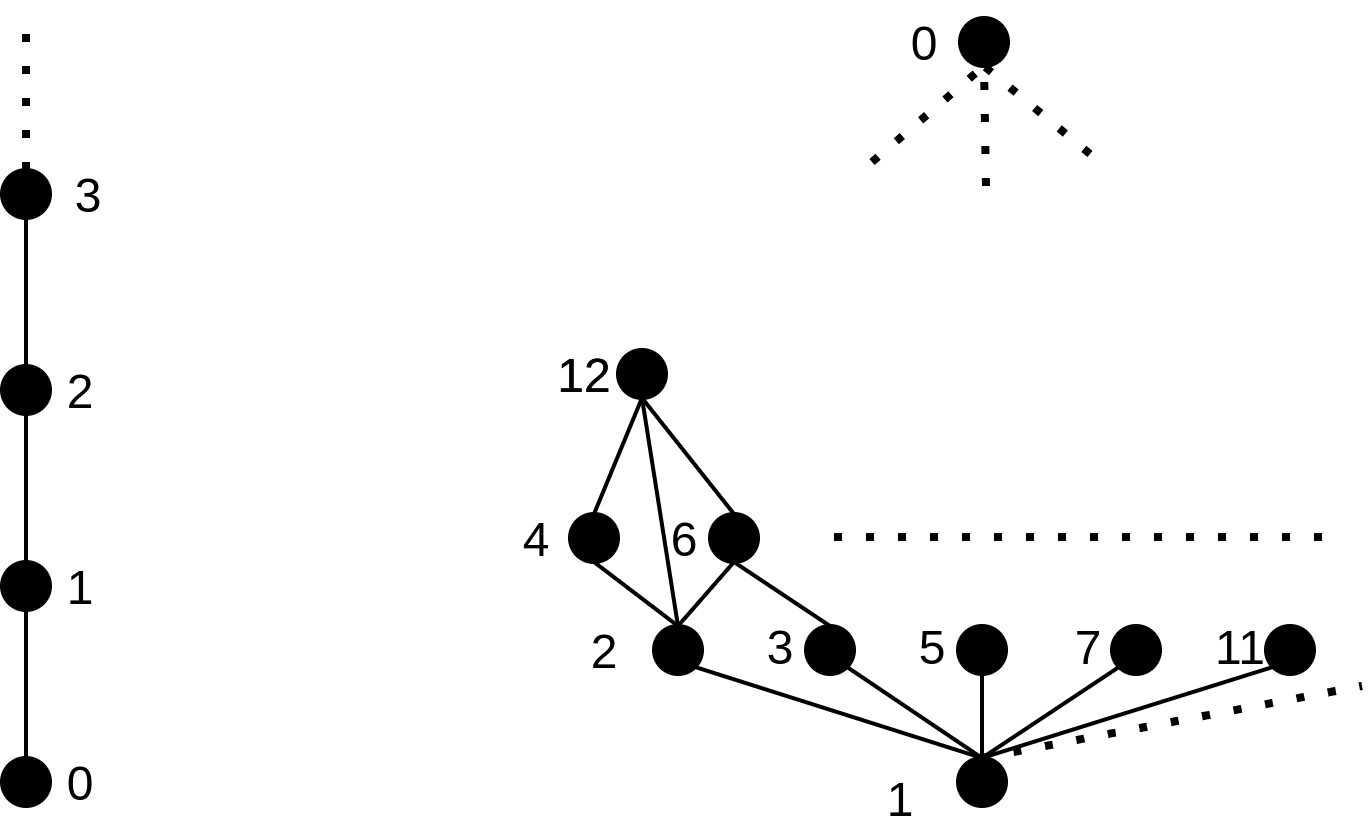
\includegraphics[width=0.5\textwidth]{images/reticolo2.png}
  \caption{Due relazioni d'ordine.}
  \label{figure:relazionireticoli}
\end{figure}

Nella Figura \ref{figure:relazionireticoli} si può vedere una rappresentazione 
(tramite reticoli, definiti a seguire) delle due relazioni d'ordine. 
La prima, quella totale, è rappresentata a destra: si può notare come sia 
``lineare'' a confronto della seconda, parziale, che è rappresentata a 
sinistra: quest'ultima infatti si dirama: alla base ha $1$, il numero che 
divide tutti gli altri; al primo ``strato'' ha tutti i numeri primi, 
il secondo i multipli dei multipli dei numeri primi (che saranno comunque collegati 
ai numeri primi, in quanto saranno divisibili anche per essi) e, commettendo 
un abuso che solitamente viene concesso, in cima vi è il numero $0$ che è divisibile 
da tutti gli altri, benché non sia divisibile per sé stesso. 

\subsubsection{Reticoli}
Un insieme $P$ con una relazione d'ordine (parziale) $\leq$, 
notato $(P, \leq)$ è detto insieme parzialmente ordinato 
o, in inglese, partially ordered set (\textit{poset}). 
L'insieme delle classi di equivalenza 
delle formule è un insieme parzialmente ordinato con delle peculiarità. 

Tra tutti i \textit{poset}, ci interessano quelli con alcune particolari proprietà 
strutturali, chiamati \textbf{reticoli}. 

\begin{figure}[!h]
  \centering 
  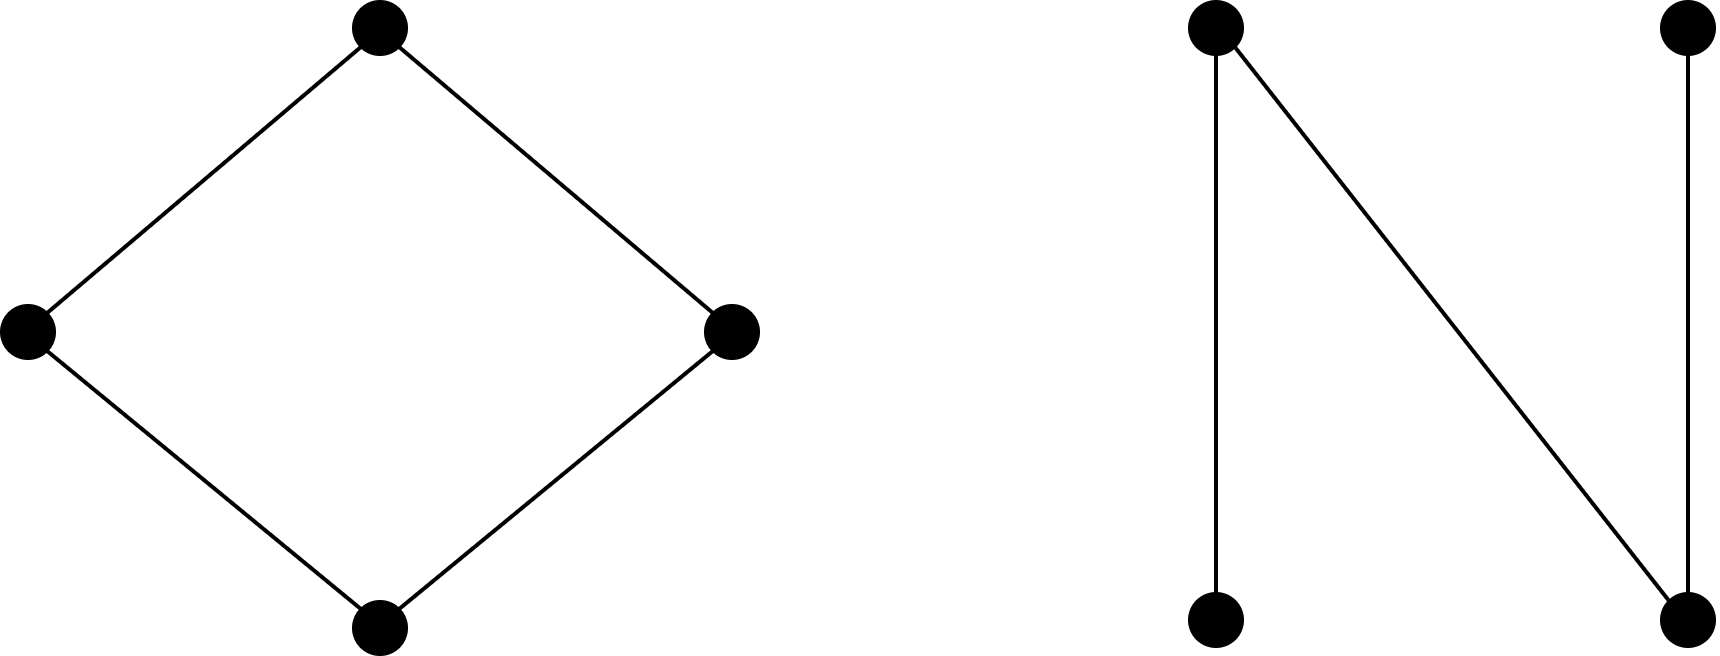
\includegraphics[width=0.5\textwidth]{images/reticolo.png}
  \caption{Due reticoli.}
  \label{figure:reticolo}
\end{figure}


La Figura \ref{figure:reticolo} riporta due immagini. 
Non entrambi sono reticoli: quello più a destra, infatti, non lo è. 
Cosa li distingue? La proprietà strutturale (più importante per i nostri 
scopi) che li divide, è che per quello più a sinistra, il reticolo, data 
ogni qualsiasi coppia di elementi possibile, si può sempre trovare 
quale dei due sia il minimo elemento che è più grande della coppia e il 
massimo elemento che è più piccolo della coppia. Questo non avviene nell'altro 
caso, infatti i due elementi ``in alto'', non hanno un minimo elemento 
più grande di loro, mentre i due elementi ``in basso'' non hanno un massimo 
elemento più piccolo di loro. In altre parole, non hanno 
\textbf{estremi inferiori} ed \textbf{estremi superiori}, che sono 
invece la proprietà fondamentale dei reticoli. 

Si definiscono quindi questi due concetti. 

\begin{defi}[Estremo inferiore]
  Dati due elementi $x, y$ appartenenti ad un insieme parzialmente ordinato $(P, \leq)$, si definisce 
  $$
  \inf(\{x,y\}) = \max\{z \in (P, \leq): z \leq x \text{ e } z \leq y\}
  $$
\end{defi}
e analogamente si definisce 
\begin{defi}[Estremo superiore]
  Dati due elementi $x, y$ appartenti ad un insieme parzialmente ordinato $(P, \leq)$, si definisce 
  $$
  \sup(\{x,y\}) = \min\{z \in (P, \leq): x \leq z \text{ e } y \leq z\}
  $$
\end{defi}
Si possono generalizzare $\inf()$ e $\sup()$ da un sottoinsieme $S \subseteq P$, con 
$P$ poset $(P, \leq)$:
\begin{align*}
  \inf(S) = \max\{z \in & (P, \leq): z \leq s\ \forall s \in S\} & \text{max dei minoranti di } S \\
  \sup(S) = \min\{z \in & (P, \leq): s \leq z\ \forall s \in S\} & \text{min dei maggioranti di } S \\
\end{align*}
A questo punto si può definire il minimo di un sottoinsieme (e analogamente il massimo), se esiste, come: 
\begin{align*}
  \min(S) := z \in S : z = \inf(S) &&
  \max(S) := z \in S : z = \sup(S)
\end{align*}
Si può ora definire formalmente un reticolo: 
\begin{defi}[Reticolo come poset]
Un reticolo è un insieme parzialmente ordinato $(R, \leq) : \forall x, y \in R$ esistono $\inf(\{x,y\})$ e $\sup(\{x,y\})$. 
\end{defi}

\noindent 
Dopo aver definito i reticoli, si definisce un'ulteriore struttura, necessaria per concludere l'argomento dell'Algebrizzazione della Logica Booleana. 

\subsection{Struttura Algebrica}
\begin{defi}
Dato un insieme $S$ e le operazioni $*_1, *_2, \cdots, *_n$ delle operazioni su $S$, allora $(S, *_1, *_2, \cdots, *_n)$ è una \textbf{struttura algebrica}.
\end{defi} 
\begin{defi}
  Visto come una struttura algebrica, un reticolo è $(R, \sqcup, \sqcap)$, con $\sqcup, \sqcap$ operazioni $\sqcup: R^2 \rightarrow R$ e $ \sqcap: R^2 \rightarrow R$, tale che le due operazioni siano commutative, associative e valga l'assorbimento.
\end{defi}
\begin{lem}
Ogni reticolo visto come insieme parzialmente ordinato è anche una struttura algebrica
$$
(R, \leq) \iff (R, \sqcup, \sqcap)
$$
\end{lem}
\begin{proof}
  ($\Longrightarrow$) con $R\equiv R,\ \forall a,b \in R$, siano:
  \begin{align*}
     a \sqcap b := \inf \{a,b\} && a \sqcup b := \sup \{a,b\}
  \end{align*}
  visto che si può verificare che per $\inf()$ e $\sup()$ valgono le proprietà di commutatività, assorbimento e associatività.
  
  ($\Longleftarrow$) con $R \equiv R$ definiamo $\forall a,b \in R$:
  \begin{align*}
    a \leq b \text{ sse } a = a \sqcap b &&
    b \leq a \text{ sse } a = a \sqcup b
  \end{align*}
  $(R, \leq)$ è quindi un poset, infatti si può verificare che $\leq$ è riflessiva, antisimmetrica e transitiva~(\ref{def:poset}). \\
  $(R, \leq)$ è anche un reticolo perché $\forall a,b \in R$ esiste $\inf$ e $\sup$: sia $c \leq a$ e $ c \leq b$
  \begin{align*}
    & c \leq a \text{ e } c \leq b \\
    \iff & c = c \sqcap a \text{ e } c = c \sqcap b & \text{per def. } \leq \\
    \iff & c = (c \sqcap b) \sqcap a \\
    \iff & c = c \sqcap (b \sqcap a) & \text{per associatività} \\
    \iff & c \leq b \sqcap a & \text{per def. } \leq \\
    \iff & c \leq \inf\{b, a\} & \text{per def. } \inf()
  \end{align*}
  Per il $\sup$ si ragiona in modo analogo. 
\end{proof}


\subsection{Definizione di Algebra Booleana}
A questo punto, siamo finalmente pronti per definire cosa sia l'Algebra Booleana.
\begin{defi}[Algebra Booleana]
L'Algebra Booleana è un sistema $(S, \sqcap, \sqcup, 0, 1, ()^c)$ di operazioni tali che $(S,\sqcup,\sqcap)$ sia un reticolo limitato, complementato, distributivo:
\begin{itemize}
  \item \textbf{limitato}: $\forall a \in S$:
    \begin{align*}
      & a \sqcup 0 = a & (a \geq 0) \\
      & a \sqcap 1 = a & (a \leq 1)
    \end{align*}
  \item \textbf{complementato}: $\forall a \in S$
    \begin{align*}
      a \sqcap a^c = 0 && a \sqcup a^c = 1
    \end{align*}
  \item \textbf{distributivo}: $\forall a,b, c \in S$:
    \begin{align*}
      a \sqcap (b \sqcup c) = (a \sqcap b) \sqcup (a \sqcap c) && a \sqcup (b \sqcap c) = (a \sqcup b) \sqcap ( a \sqcup c)
    \end{align*}
\end{itemize}
\end{defi}

Un esempio è il seguente: dato un insieme $A$ si consideri 
$(P(A), \cup, \cap, \emptyset, A, ()^c)$ e si ha 
$(P(A), \subseteq)$ tale che $A \subseteq B \iff A = A \cap B$. 

\paragraph{Esercizio}
Si dimostri che le seguenti sistemi siano un'algebra booleana:
\begin{itemize}
  \item $(F(A), \cup, \cap, \emptyset, A, ()^c)$ \\
    con $A$ un insieme infinito, e $F(A)$ l'insieme dei suoi sottoinsiemi finiti o complementi di insiemi finiti
  \item $(\{0,1\}, \min, \max, 0, 1, 1-\_)$
\end{itemize}

\subsubsection{Algebra di Lindenbaum}
L'algebra delle formule, chiamata anche \textbf{Algebra di 
Lindenbaum delle Formule}, è definita come 
$$
(\mathscr{F_L}/_{\equiv}, \land, \lor, \bot, \top, \neg)
$$
Dato che $\equiv$ è una congruenza, si possono definire le seguenti operazioni con $A,B \in \mathscr{F_L}$:
\begin{align*}
  [A]_{\equiv} \land [B]_{\equiv} & = [A \land B]_{\equiv} \\
  [A]_{\equiv} \lor [B]_{\equiv} & = [A \lor B]_{\equiv} \\
  [A]_{\equiv} \rightarrow [B]_{\equiv} & = [A \rightarrow B]_{\equiv} \\
  \neg [A]_{\equiv} & = [\neg A]_{\equiv} \\
  [\top]_{\equiv} & = \text{ tautologie} \\
  [\bot]_{\equiv} & = \text{ contraddizioni} \\
\end{align*}
La cardinalità dell'insieme delle classi di equivalenza scrivibili con $n$ variabili è:
$$
|\mathscr{F_L}^{(n)}/_\equiv| = 2 ^ {2^n} = |\{F: \{0,1\}^n \rightarrow \{0,1\}\}| = |\mathscr{P}(\{1,\cdots,2^n\})|
$$

\subsection{Funzioni Termine}
Al fine di arrivare ad un discorso completo sulle Forme Normali, si continua a ragionare sulle classi d'equivalenza delle formule e la loro struttura, ora da un punto di vista che sembra essere diverso ma che in conclusione si riunirà con quanto detto precedentemente. 

Si rifletta sul significato di 
\begin{align}
\label{fun:formula-computazionale}
\models F \iff \forall \mathcal{v}: \mathscr{L} \rightarrow \{0,1\},\ \mathcal{v}(F) = 1
\end{align}
in termini ``computazionali'' significa \textit{tenere fermo} l'argomento ($F$) e far cambiare le funzioni. Sarebbe comodo scambiare i ruoli: la formula si comporta come una funzione che prende come argomenti gli assegnamenti.

Siano $A \in \mathscr{F_L}$ una formula e $n \in \mathbb{N}$. Le lettere proposizionali che occorrono in $A$ si indicano con
$$
Var(A) \subseteq \mathscr{L} \subseteq \{p_1, p_2, \cdots, p_n\}
$$
Sia ora $\hat{A}$ una \textbf{funzione termine} $\hat{A} : \{0,1\}^n \rightarrow \{0,1\}$ tale che:
$$
\forall \mathcal{v}:\mathscr{L} \rightarrow \{0,1\},\ \hat{A}(\mathcal{v}(p_1), \mathcal{v}(p_2), \cdots, \mathcal{v}(p_n)) = \widetilde{\mathcal{v}}(A)
$$

\begin{defi}[Funziona Termine]
Definizione di $\hat A : \{0,1\}^n \rightarrow \{0,1\}$ induttiva su $A$:
\begin{itemize}
  \item \textbf{base}: Se $ A = p_i$, con $p_i \in \{p_1, p_2, \cdots, p_n\}$ un letterale:
  $$\hat A := \hat{p_i} : \{0,1\}^n \rightarrow \{0,1\}$$
  con $\hat{p_i}(t_1, \cdots, t_n) = t_i$, l'$i$-esima proiezione. 
  Quindi $\forall \mathcal{v}: \mathscr{L} \rightarrow \{0,1\}$ si verifica che: 
  $$
  \hat{A} = \hat{p_i}(\mathcal{v}(p_1), \cdots, \mathcal{v}(p_n)) = \mathcal{v}(p_i) = \widetilde{\mathcal{v}}(p_i) = \widetilde{\mathcal{v}}(A)
  $$
\item \textbf{passo}: $\forall (t_1, \cdots, t_n) \in \{0,1\}^n$
  \begin{itemize}
    \item Se $A = \neg B$: $\hat{A}(t_1, \cdots, t_n) =  1 - \hat{B}(t_1, \cdots, t_n)$
    \item Se $A = B \land C$: $\hat{A}(t_1, \cdots, t_n) = \min \{\hat{B}(t_1, \cdots, t_n),\ \hat{C}(t_1, \cdots, t_n)\}$
    \item Se $A = B \lor C$: $\hat{A}(t_1, \cdots, t_n) = \max \{\hat{B}(t_1, \cdots, t_n),\ \hat{C}(t_1, \cdots, t_n)\}$
    \item Se $A = B \rightarrow C$: $\hat{A}(t_1, \cdots, t_n) = \max \{1 - \hat{B}(t_1, \cdots, t_n),\ \hat{C}(t_1, \cdots, t_n)\}$
  \end{itemize}
\end{itemize}
\end{defi}
\noindent
Ora si possono vedere come \textit{funzioni termine} la riflessione iniziale~(\ref{fun:formula-computazionale}): 
$$
\models F \iff \hat{F}(t_1, \cdots, t_n) = 1,\ \forall (t_1, \cdots, t_n)
$$
e l'equivalenza logica: 
$$
[F]_{\equiv} = [G]_{\equiv} \iff F \equiv G \iff \hat{F}(t_1, \cdots, t_n) = \hat{G}(t_1, \cdots, t_n),\ \forall t_i \in \{0,1\}^n
$$
Allo stesso modo si può dare una definizione diversa di Algebra Booleana, \textit{isomorfa} all'Algebra di Lindenbaum.
\begin{defi}[Algebra Booleana su Funzioni Termine sui primi $n$ termini]
$$
\hat{\mathscr{F}}_\mathscr{L}^{(n)} = (\{\hat{A}: \{0,1\}^n \rightarrow \{0,1\}, A \in \mathscr{F_L}\}, \land, \lor, \neg, \bot, \top) 
$$
dove i significati degli operatori sono quelli espressi nella definizione di funzioni termine. 
\end{defi}

\subsection{Teorema di Completezza Funzionale}
Concentriamoci sull'algebra $\hat{\mathscr{F}}_\mathscr{L}^{(n)}$ appena espressa e una $Funz^{(n)}$ definita come:
$$
Funz^{(n)} = (\{f: \{0,1\}^{(n)} \rightarrow \{0,1\}\}, \land, \lor, \neg, \bot, \top)
$$
Che rapporto sussiste tra le due Algebre?
Per ogni $n \in \mathbb{N}$, la prima ha come universo l'insieme di tutte le Funzioni Termine per ogni formula $A \in \mathscr{F_L}$, mentre la seconda ha come universo tutte le funzioni $f: \{0,1\}^n \rightarrow \{0,1\}$. \\
Sicuramente, data la restrizione, si può affermare che:
$$
\hat{\mathscr{F}}_\mathscr{L}^{(n)} \subseteq Funz^{(n)}
$$
Si dimostra, ora, che vale anche:
$$
\hat{\mathscr{F}}_\mathscr{L}^{(n)} \supseteq Funz^{(n)}
$$
Questo fatto prende il nome di \textbf{Teorema di Completezza Funzionale}. 
A parole, ciò che afferma è che ogni funzione $f: \{0,1\}^n \rightarrow \{0,1\}$ è esprimibile come una formula $F \in \mathscr{F_L}$. \\
Chiaramente, se dimostrato, vuol dire che le due algebre sono in realtà \textit{isomorfe}. 
\begin{teo}[di Completezza Funzionale]
$$
  \mathscr{\hat{F}_L}^{(n)} \supseteq Funz^{(n)},\ \forall n \in \mathbb{N}
$$
\end{teo}

La dimostrazione consiste nel fornire per ogni $n \in \mathbb{N}$ e ogni funzione $f: \{0,1\}^{n} \rightarrow \{0,1\}$ una formula \textit{costruibile} $F \in \mathscr{F_L}^{(n)} : f = \hat F$. 
\begin{proof}
Sia $f: \{0,1\}^{n} \rightarrow \{0,1\}$ una funzione, la cui cardinalità del dominio è $2^{n}$. Per ogni combinazione degli $n$ argomenti $(a_{i_1}, a_{i_2}, \cdots, a_{i_n})$ esiste un valore $b_i \in \{0,1\}$ associato:
\begin{align}
  f :=
  \begin{cases}
    (a_{1_1}, a_{1_2}, \cdots, a_{1_j}, \cdots, a_{1_n}) & \longrightarrow b_1 \\
    (a_{2_1}, a_{2_2}, \cdots, a_{2_j}, \cdots, a_{2_n}) & \longrightarrow b_2 \\
    ~~~~~~~~~~~~~~~     \vdots           & ~~~~~~~~ \vdots \\
    (a_{i_1}, a_{i_2}, \cdots, a_{i_j}, \cdots, a_{i_n}) & \longrightarrow b_i \\
    ~~~~~~~~~~~~~~~     \vdots           & ~~~~~~~~ \vdots \\
    (a_{(2^n)_1}, a_{(2^n)_2}, \cdots, a_{(2^n)_j}, \cdots, a_{(2^n)_n}) & \longrightarrow b_{(2^n)}
  \end{cases}
\end{align}
Costruiamo una formula $F \in \mathscr{F_L}$ in modo tale che $ \hat{F} = f$.
\begin{itemize}
  \item se $f(t_1, \cdots, t_n) = 0$ per ogni $(t_1, \cdots, t_n)$: $F = \bot$
  \item altrimenti sia $I \subseteq \{1, 2, \cdots, 2^{n}\}$ tale che:
  $$
  i \in I \iff b_i = 1
  $$
  (intuitivamente, $I$ contiene i numeri delle ``righe'' della tabella di verità della funzione $f$ in cui l'immagine è il numero $1$). \\
  Per ogni $i \in I$ si considera la $i$-esima tupla $(a_{i_1}, a_{i_2}, \cdots, a_{i_n})$ di argomenti di $f$. \\
  Per ogni $j \in \{1, \cdots, n\}$ si definisce:
  \begin{align*}
  A_{ij} =
  \begin{cases}
    p_j & \text{se } a_{ij} = 1 \\
    \neg p_j & \text{se } a_{ij} = 0
  \end{cases} &&
  \text{con } A_{ij} \in \mathscr{F_L}^{(n)}
  \end{align*}
  Si pone $F = \bigvee\limits_{i \in I}\bigwedge\limits_{j \in n} A_{ij}$
  
  Si mostra che $\hat{F} = f$, ovvero che per ogni riga $i \in I$:
  $$
  {[ \bigwedge\limits_ {j = 1}^{n} \hat{A}_{ij}(t_1, \cdots, t_n) ]} = 1
  \iff (t_1, \cdots, t_n) = (a_{i_1}, \cdots, a_{i_n})
  $$
  Infatti
  \begin{itemize}
  \item se $(t_1, \cdots, t_n) = (a_{i_1}, \cdots, a_{i_n})$, $\forall j \leq  n$:
    \begin{align*}
      \hat A_{ij}(t_1, \cdots, t_n) = t_j =
      \begin{cases*}
        \mathcal{v}(p_j) = a_{i_j} \\
        \mathcal{v}(\neg p_j) = 1 - a_{i_j}
      \end{cases*}
      &
      \begin{rcases*}
        \text{ se } a_{i_j} = 1 \\
        \text{ se } a_{i_j} = 0
      \end{rcases*} = 1
    \end{align*}
  \item se $(t_1, \cdots, t_n) \neq (a_{i_1}, \cdots, a_{i_n})$, $\exists t_j \neq a_{i_j}$:
    \begin{align*}
      \hat A_{ij}(t_1, \cdots, t_n) = t_j =
      \begin{cases*}
        \mathcal{v}(p_j) = a_{i_j} \\
        \mathcal{v}(\neg p_j) = 1 - a_{i_j}
      \end{cases*}
      &
      \begin{rcases*}
        \text{ se } a_{i_j} = 0 \\
        \text{ se } a_{i_j} = 1
      \end{rcases*} = 0
    \end{align*}
  \end{itemize}
  Quindi $(A_{i_1} \land A_{i_2} \land \cdots \land A_{i_n})$ può essere resa vera solo da un assegnamento. In definitiva, 
  $$
  \hat{F} = \bigvee\limits_{i\in I}\bigwedge\limits_{j}^n \hat A_{i_j}(t_1, \cdots, t_n) = 1 \iff (t_1, \cdots, t_n) \text{ è la riga } i \text{-esima, e } i \in I
  $$
  Quindi $\hat F = f$.  
\end{itemize}
\end{proof}

\subsubsection{Considerazioni sul Teorema di Completezza Funzionale}
Per come è stato provato il Teorema di Completezza Funzionale, la funzione termine si può anche esprimere come: 
$$
G = \bigwedge\limits_{i \in J} \bigvee_{j = 1}^{n} B_{ij}
$$
con
\begin{align*}
  J \subseteq \{0, \cdots, 2^n-1\} &&
  i \in J \iff b_j = 0 &&
  B_{ij} =
  \begin{cases}
    \neg p_j & a_{ij} = 1 \\
    p_j & a_{ij} = 0 \\
  \end{cases}
\end{align*}
Si ha, quindi, che $\hat{F} = f = \hat{G}$\footnote{Ciò che è stato fatto è esattamente uguale alla costruzione dei minterm e maxterm per una data tavola di verità.}, il che è una dimostrazione che una qualsiasi formula può essere messa in una \textbf{forma normale} perché $\hat{\mathscr{F}}_\mathscr{L}^{(n)} = Funz^{(n)}$.

Sebbene il Teorema possa sembrare banale, in quanto la sua dimostrazione è
semplice, il suo contenuto non è nullo né scontato. Un esempio di mancanza 
funzionale è già presente nella Logica Proposizionale stessa, nonostante 
la dimostrazione precedente, rimuovendo il vincolo su $n$ e definendo
$$
Funz^{\omega} := \{f:\{0,1\}^{\omega} \rightarrow \{0,1\}\}
$$
con $\omega = |\mathbb{N}|$, in altre parole l'insieme di tutte le successioni 
infinite di valori $\{0,1\}$. Se valesse il Teorema di Completezza Funzionale 
anche in questo caso, si dovrebbe poter affermare che tale insieme 
è incluso nelle classi di equivalenza scritte nelle classi di equivalenza 
delle formule scritte con $\omega$ variabili: 
$$
Funz^{\omega} \subseteq \hat{\mathscr{F}}_\mathscr{L}^{\omega} = \mathscr{F_L}^{\omega}/_\equiv
$$
Ma in realtà
$$
|Funz^{\omega}| = |\mathbb{R}| \geq |\mathbb{N}| = |\mathscr{F_L}^{\omega}/_\equiv|
$$
e pertanto non è valido. 

\paragraph{Forme Normali Canoniche}
Le forme normali che abbiamo trovato non sono desiderabili per gli scopi 
futuri, in quanto sono molto prolisse: ognuno degli $A_{ij}$ menziona 
tutte le lettere proposizionali $p_1, \cdots, p_n$ (analogamente per le 
forme congiuntive) ed è infatti chiamata Forma Normale Disgiuntiva (or di and) \textbf{Canonica} o \textbf{Completa}. \\
Si noti la prolissità nel costruire una $F \in \mathscr{F_L}$ t.c. $\hat F = f : \{0, 1\}^3 \rightarrow \{0, 1\}$ con: 
$$
f(t_1, t_2, t_3) = t_1 ~~~ \forall (t_1, t_2, t_3)
$$
È chiaro che la formula più ``corta'' è $F = t_1$, ma con la forma 
canonica si rappresenta come:
$$
F = (p_1 \land \neg p_2 \land \neg p_3) \lor (p_1 \land \neg p_2 \land p_3) \lor (p_1 \land p_2 \land \neg p_3) \lor (p_1 \land p_2 \land p_3)
$$

\paragraph{Insieme funzionalmente completo di connettivi}
C'è un'altra nozione, legata alla Completezza Funzionale, che è molto interessante, 
ossia la nozione di \textit{insieme funzionalmente completo di connettivi}. 
\begin{defi}[Insieme funzionalmente completo di connettivi]
Un insieme 
  $$
  C \subseteq \{\land, \lor, \rightarrow, \neg, \leftrightarrow, \bot, \top\}
  $$
è definito \textit{funzionalmente completo} se per ogni $F \in \mathscr{F_L}$ esiste una $G \in \mathscr{F_L}$ scritta usando solo i connettivi in $C$ tale che $F \equiv G$ e $\hat{F} = \hat{G}$, ossia $[F]_{\equiv} = [G]_{\equiv}$. 
\end{defi}

Un insieme di connettivi funzionalmente 
completo è dato dal Teorema di Completezza Funzionale stesso, ossia 
$C = \{\land, \lor, \neg\}$. Si può mostrare facilmente che 
anche $\{\neg, \land\}$ e $\{\neg, \lor\}$ sono completi (in quanto, grazie alle 
leggi di De Morgan, $(A \lor B) = \neg (\neg A \land \neg B)$). Questi non 
sono gli unici insiemi funzionalmente completi: 
$\{\neg, \rightarrow\}$ (in quanto $(A \land B) \equiv \neg (A \rightarrow \neg B)$ 
e $(A \lor B) \equiv ((\neg A) \rightarrow B)$ 
e $\{\rightarrow, \bot\}$. In particolare, un insieme composto da un 
solo connettivo, il \texttt{nand}, è anch'esso funzionalmente completo, 
in quanto ogni altro connettivo è ricostruibile utilizzando solo 
$$
A \barwedge B = \neg (A \land B)
$$
infatti $\neg A \equiv A \barwedge A$ e, ovviamente, $A \land B \equiv \neg ( A \barwedge B)$ 
per definizione. 

\section{Forme Normali}
Dopo averle introdotte col Teorema di Completezza Funzionale, possiamo 
passare ad un esame più approfondito delle Forme Normali.
Le Forme Normali Congiuntive e Disgiuntive Canoniche sono 
esageratamente prolisse. Sarebbe utile conservare l'idea delle Forme Normali 
con formule più succinte. 

\subsection{Forma Normale Negata}
Una terza forma normale, chiamata \textbf{Negation 
Normal Form} (NNF) che, per definizione, è l'insieme delle formule 
che rispettano le seguenti proprietà: 
\begin{itemize}
  \item non contiene $\rightarrow$ 
  \item $\neg$ occorre solo applicato a lettere proposizionali
\end{itemize}
quindi, per esempio 
\begin{align*}
p_1 \land \neg(p_2 \lor p_3) \notin NNF \\
p_1 \land (\neg p_2 \lor \neg p_3) \in NNF
\end{align*}

\begin{defi}[Sottoformula]
$G$ è sottoformula di $F$ sse $G$ occorre in ogni $\mathscr{L}$-costruzione di $F$ e si indica con $G \preccurlyeq F$
\end{defi}

\begin{lem}
Ogni formula $F \in \mathscr{F_L}$ è equivalente a una $F^{N} \in NNF$. 
\end{lem}
\begin{proof}
Per provare il lemma, descriviamo come trasformare $F$ in $F^{N}$ in un numero 
finito di passi, dove ogni passo produce una formula equivalente alla precedente. 
Per ottenere la sequenza si applica ad ogni passo una delle seguenti 
trasformazioni a $G \preccurlyeq F$:

\begin{enumerate}
  \item $C \rightarrow D \leadsto (\neg C) \lor D$
  \item $\neg \neg C \leadsto C$
  \item $\neg(C \lor D) \leadsto \neg C \land \neg D$
  \item $\neg (C \land D) \leadsto \neg C \lor \neg D$
\end{enumerate}

Un'osservazione preliminare su questo algoritmo è che si può mostrare che applicando 
le quattro regole in un ordine qualsiasi si ottiene sempre $F^{N} \in NNF$. 
Si mostrerà che partendo da $(1)$ e applicando le altre trasformazioni si possa 
arrivare a $F^{N}$: sia data $F \in \mathscr{F_L}$. In un numero finito di applicazioni 
di $(1)$ si ottiene una $F'$ in IFNF (Implication-Free Normal Form), equivalente 
a $F$. 

Si introduce una misura di \textit{distanza}: si definisce 
$i(E)$ come il numero di connettivi $\rightarrow$ nella formula $E$. 
Si ha, quindi, 
che $E \in IFNF \iff i(E) = 0$. Inoltre, se $E \notin IFNF$, allora 
$E'$ ottenuta applicando $(1)$ su $E$ deve avere $i(E) > i(E')$.\\
È chiaro che $F \equiv F'$ poiché l'applicazione di $(1)$ è semplicemente 
l'applicazione di una equivalenza eseguita grazie al Teorema di Sostituzione. 
Quindi, in un certo numero di passi  si ha
$$ 
F = F_0 \equiv \cdots \equiv F' (\in IFNF) \equiv F_i \equiv \cdots \equiv F_n (\in NNF)
$$
e si nota che le applicazioni di $(2)$, $(3)$ e $(4)$ trattano tutte equivalenze logiche. Ciò che bisogna dimostrare è che la sequenza di trasformazioni termini, ossia l'algoritmo non è infinito ($n \in \mathbb{N}$).

Per dimostrare che l'algoritmo termina, siano ora $A,E \in \mathscr{F_L}$ e si definisce $\ell(A) = $ ``n° di occorrenze di connettivi in $A$''.
Definiamo quindi $m(E)$ come la somma del numero di connettivi presenti nelle sottoformule $\neg A$ di $E$: 
$$
m(E) = \sum_{\neg A \preccurlyeq E} \ell(A)
$$
Si noti che 
$$
m(E) = 0 \iff E \in NNF
$$
Infatti:
\begin{itemize}
  \item  se $E \in NNF$:
    \begin{align*}
      & \forall \neg A \preccurlyeq E,\ A \in \mathscr{L} & \text{per def. } NNF\\
      \iff & \forall \neg A \preccurlyeq E,\ \ell(A) = 0 \\
      \iff & m(E) = 0
    \end{align*}
  \item se $m(E) = 0$:
    $$
    \sum_{\neg A \preccurlyeq E} \ell(A) = 0 \iff \forall \neg A \preccurlyeq E,\ \ell(A) = 0 \iff \forall \neg A \preccurlyeq E,\ A \in \mathscr{L}
    $$ 
\end{itemize}
In un passaggio eseguito con una delle $(2), (3), (4)$ generando 
$$
E \leadsto E'
$$
si ha che $m(E) > m(E')$. Se si riesce a dimostrare quest'ultima affermazione, 
allora si dimostra automaticamente che il procedimento termina in un numero 
finito di passi. 
\paragraph{(2) $\neg \neg C \leadsto C$}: In questo caso
\begin{align*}
  \begin{cases}
        m(\neg \neg C) & = \ell(\neg C) + m(\neg C)
                         = \ell(C) + 1 + \ell(C) + m(C) \\
                       & = 1 + 2 \cdot \ell(C) + m(C) \\
        m(C)
  \end{cases}
\end{align*}
$$
  \implies m(\neg \neg C) > m(C)
$$

\paragraph{(3) $\neg (C \lor D) \leadsto \neg C \land \neg D$}: In questo caso
\begin{align*}
  \begin{cases}
    m(\neg (C \lor D)) & = \ell(C \lor D) + m(C) + m(D) \\
                       & = \ell(C) + \ell(D) + m(C) + m(D) + 1 \\
    m(\neg C \land \neg D) 
                       & = \ell(C) + \ell(D) + m(C) + m(D)
  \end{cases}
\end{align*}
$$
  \implies m(\neg (C \lor D)) > m(\neg C \land \neg D)
$$
Analogamente per $(4)$.

Data una formula $F \in \mathscr{F_L}$, si può costruire una successione 
finita 
$$ 
F = F_0 \equiv \cdots \equiv F' (\in IFNF) \equiv F_i \equiv \cdots \equiv F_n (\in NNF)
$$
e ovviamente $F \equiv F_n$, per un qualche $n \in \mathbb{N}$. 
\end{proof}

\subsection{Forma Normale Congiuntiva e Disgiuntiva}
Le CNF o FNC, Forme Normali Congiuntive, sono un sovrainsieme delle CNF \textit{complete} o canoniche.
\begin{defi}[Letterale]
Un \textit{letterale} è una formula nella forma $p$ o $\neg p$ per qualche lettera proposizionale $p$ (i.e., o è una lettera proposizionale o è la sua negata).
La definizione di \textbf{letterale opposto} a uno dato è, dato $A$ letterale, l'opposto di $A$:
$$
\bar{A} = 
\begin{cases}
  \neg p & \text{se } A = p \\
  p & \text{se } A = \neg p
\end{cases}
$$
\end{defi}
\begin{defi}[Clausola]
Una \textit{clausola} è una disgiunzione di un numero finito $k$ di letterali:
$$
\ell_1 \lor \ell_2 \cdots \lor \ell_k
$$
dove ogni $\ell_i$ è un letterale. 
\end{defi}
\begin{defi}[CNF o FNC]
Una \textbf{forma normale congiuntiva} è una congiunzione di un numero finito $h$ di 
clausole: 
$$
C_1 \land C_2 \land \cdots \land C_h
$$
dove ogni $C_j$ è una clausola. 
\end{defi}
\begin{defi}[Clausola vuota]
Una \textbf{clausola vuota} $\qedsymbol$ è definita come la disgiunzione 
di zero letterali. 
\end{defi}

Questo concetto è importante e non va confuso col concetto 
di \textbf{CNF vuota} $\emptyset$, definita come la congiunzione di zero clausole. 
Prendendo una sequenza di letterali e formule
\begin{align*}
F_0 & = \qedsymbol \\
F_1 & = \ell_1 \\
F_2 & = \ell_1 \lor \ell_2 \\
F_3 & = \ell_1 \lor \ell_2 \lor \ell_3 \\
\vdots \\
F_i & = \ell_1 \lor \ell_2 \lor \ell_3 \lor \cdots \lor \ell_i
\end{align*}
possiamo notare che ogni assegnamento che soddisfa una formula $F_i$, soddisfa anche quella successiva $F_{i+1}$. Per questo $F_i \rightarrow F_{i+1}$ è una tautologia. \\
Seguendo questa definizione la clausola vuota è insoddisfacibile e pertanto è $\qedsymbol \equiv \bot$.

Per l'insieme di CNF vuote, si ha 
\begin{align*}
& \emptyset \\
& C_1 \\
& C_1 \land C_2 \\
& C_1 \land C_2 \land C_3\\
& \vdots \\
& C_1 \land C_2 \land C_3 \land C_4
\end{align*}
qui, al contrario, ogni assegnamento che soddisfa una clausola $C_i$, soddisfa anche la precedente $C_{i-1}$. \\
Seguendo questa definizione la CNF vuota è soddisfacibile ed è, in realtà, soddisfatta da ogni assegnamento: $\emptyset \equiv \top$. 

\begin{defi}[DNF o FND]
Una \textit{forma normale disgiuntiva} è una disgiunzione di un numero finito $n$ di formule:
$$
D_1 \lor D_2 \lor \cdots \lor D_n
$$
dove ogni $D_i$ è una congiunzione chiamata \textbf{co-clausola} di un numero finito $v$ di letterali:
$$
\ell_1 \land \ell_2 \land \cdots \land \ell_v
$$
\end{defi}

DNF si tratta, quindi, di una struttura duale rispetto alle CNF.
Si noti la terminologia speciale per le CNF: questa terminologia è riservata alle CNF in quanto la dualità tra CNF e DNF verrà spezzata. 

\begin{lem}
Ogni formula $F \in \mathscr{F_L}$ è logicamente equivalente a una formula $F^c \in CNF$ 
e a una formula $F^d \in DNF$.
\end{lem}

Questo è già stato dimostrato grazie al teorema di completezza funzionale, che tuttavia utilizzava le CNF e DNF complete. 
\begin{proof}[esistenza DNF/CNF]
Per induzione strutturale su $F$:
\begin{itemize}
  \item \textbf{base}: se $F = p$ con $p \in \mathscr{L}$ allora $p = p^c = p^d$.
  \item \textbf{passo}:
    \begin{itemize}
      \item se $F = \neg G$, per ipotesi induttiva si ha $G^c \equiv G$ e $G^d \equiv G$. 
        Allora, se
        \begin{align*}
           G = C_1 \land C_2 \land \cdots \land C_h &&
          \text{dove ogni } C_i = \ell_{i_1} \lor \cdots \lor \ell_{i_{k_i}}
        \end{align*}
        si ha che:
        \begin{align*}
          \neg G \equiv \neg (G^c) & \equiv \neg (C_1 \land \cdots \land C_h) \\
                   & \equiv \neg C_1 \lor \neg C_2 \lor \cdots \lor \neg C_h := (\neg G)^d & \text{per DeMorgan}
        \end{align*}
        \begin{align*}
          \text{dove ogni } \neg C_i & \equiv \neg (\ell_1 \land \ell_2 \land \cdots \land \ell_v) \\
                               & \equiv \neg \ell_{i_1} \land \cdots \land \neg \ell_{i_{k_i}} & \text{per DeMorgan} \\
                               & \equiv \bar \ell_{i_1} \land \cdots \land \bar \ell_{i_{k_i}} & \neg \ell_{i_j} \text{ è } \equiv \text{ a un letterale opposto} \\
          \implies (\neg G)^d \in DNF 
        \end{align*}
        e similmente:
        \begin{align*}
          \neg G \equiv \neg (G^d) & \equiv \neg (D_1 \lor \cdots \lor D_n) \\
                   & \equiv \neg D_1 \land \neg D_2 \land \cdots \land \neg D_n := (\neg G)^c & \text{per DeMorgan}
        \end{align*}
        \begin{align*}
          \text{con } \neg D_i & \equiv \neg (\ell_{i_1} \land \cdots \land \ell_{i_{k_i}}) \\
                               & \equiv \neg \ell_{i_1} \land \cdots \land \neg \ell_{i_{v_i}} & \text{per DeMorgan} \\
                               & \equiv \bar \ell_{i_1} \land \cdots \bar \neg \ell_{i_{v_i}} & \neg \ell_{i_j} \text{ è } \equiv \text{ a un letterale opposto} \\
          \implies (\neg G)^c \in CNF 
        \end{align*}
        Quindi esistono sia $F^d := (\neg G)^d \equiv \neg (G^c)$ che $F^c := (\neg G)^c \equiv \neg (G^d)$. 
      \item se $F = (G \land H)$, per ipotesi induttiva si ha:
        \begin{align*}
           G^c \equiv G && G^d \equiv G \\
           H^c \equiv H && H^d \equiv H
        \end{align*}
        Si definisce, allora
        \begin{itemize}
          \item $F \equiv F^c$ \\
                con $F^c := (G^c \land H^c)$ e, banalmente $(G^c \land H^c) \in CNF$
          \item $F^d$:
            \begin{align*}
              F & \equiv (G^d \land H^d) \\ 
                & \equiv (G_1 \lor \cdots \lor G_u) \land (H_1 \lor \cdots \lor H_v) \\
                & \equiv \bigvee\limits_{i,j}(G_i \land H_j) & \text{per Distributività Generalizzata}~(\ref{def:distributibilita-generalizzata})
            \end{align*}
            Ma visto che $C_i$ e $H_j$ sono \textit{co-clausole}, anche $(G_i \land H_j)$ lo è.
            $$
            \implies F^d := \bigvee\limits_{i=1}^u \bigvee\limits_{j=1}^v (G_i \land H_i) \in DNF
            $$
        \end{itemize}
      \item se $F = (G \lor H)$, per ipotesi induttiva si ha:
        \begin{align*}
          G^c \equiv G && G^d \equiv G \\
          H^c \equiv H && H^d \equiv H
        \end{align*}
        Si definisce, allora
        \begin{itemize}
          \item $F \equiv F^d$ \\
                con $F^d := (G^d \lor H^d)$ e, banalmente $(G^d \lor H^d) \in DNF$
          \item $F^c$:
            \begin{align*}
              F & \equiv (G^c \lor H^c) \\ 
                & \equiv (G_1 \land \cdots \land G_u) \lor (H_1 \land \cdots \land H_v) \\
                & \equiv \bigwedge\limits_{i,j}(G_i \lor H_j) & \text{per Distributività Generalizzata}~(\ref{def:distributibilita-generalizzata})
            \end{align*}
            Ma visto che $C_i$ e $H_j$ sono \textit{clausole}, anche $(G_i \lor H_j)$ lo è.
            $$
            \implies F^c := \bigwedge\limits_{i=1}^u \bigwedge\limits_{j=1}^v (G_i \lor H_i) \in CNF
            $$generalizzata
        \end{itemize}       
      \item se $F = (G \rightarrow H)$, ci si comporta analogamente contando che $F \equiv (\neg G \lor H)$      
    \end{itemize}
\end{itemize}
\end{proof}

Si nota, tuttavia, che muoversi tra DNF e CNF con la distributività generalizzata causa un notevole allungamento delle formule. Per esempio:
\begin{align*}
        \bigvee\limits_{i = 1}^{n} (p_i \land q_i) \equiv \bigwedge\limits_{i = 1}^{2^n}(\ell_{i_1} \lor \cdots \lor \ell_{i_n})
\end{align*}
quindi c'è una dilatazione esponenziale. Questo è un bel problema.


Ci sono algoritmi più intelligenti per generare da DNF delle formule CNF più corte? \\
Purtroppo no. 
